%\documentclass[twoside,12pt]{article}% dvoustranný tisk
\documentclass[twoside,12pt]{book}% jednostranný tisk

\usepackage[english]{babel}
\usepackage[utf8x]{inputenc}
\PrerenderUnicode{ěščřžýáíéĚŠČŘŽÝÁÍÉďťňĎŤŇůúÚóÓ}

\usepackage{amssymb}
\usepackage{amsmath}
\usepackage{pdfpages}
\usepackage{hyperref}
\usepackage{amsthm}
%\usepackage{subfig}
\usepackage{bm}
\usepackage{float}
%\usepackage{subfig}
\usepackage{wrapfig}
\usepackage{caption}
\usepackage{mathtools} %symboly nad sipkami
\usepackage{placeins} %\floatbarrier
\usepackage{mathtools}
\usepackage{rotating} % pro sidewaystable
\usepackage{siunitx}
\usepackage{multirow}
\usepackage{epstopdf}
\usepackage{enumerate}
\usepackage{tabularx}
\usepackage{subcaption}
	\renewcommand{\arraystretch}{1.4}
	\usepackage{array}
	\newcolumntype{C}[1]{>{\centering\let\newline\\\arraybackslash\hspace{0pt}}m{#1}}	% center normal
	\newcolumntype{S}[1]{>{\small\centering\let\newline\\\arraybackslash\hspace{0pt}}m{#1}}	% center small
	\newcolumntype{L}[1]{>{\small\raggedright\let\newline\\\arraybackslash\hspace{0pt}}m{#1}} % small left
	\newcolumntype{R}[1]{>{\small\raggedleft\let\newline\\\arraybackslash\hspace{0pt}}m{#1}} % small right
	\newcolumntype{F}[1]{>{\footnotesize\raggedright\let\newline\\\arraybackslash\hspace{0pt}}m{#1}} % footnotesize right
	\newcolumntype{D}[1]{>{\footnotesize\raggedleft\let\newline\\\arraybackslash\hspace{0pt}}m{#1}} % footnotesize left
	\newcolumntype{G}[1]{>{\footnotesize\centering\let\newline\\\arraybackslash\hspace{0pt}}m{#1}}	% center footnotesize
\usepackage{booktabs} % package na tvorbu peknych tabulek 

\usepackage{graphicx}
\DeclareGraphicsExtensions{.png,.pdf,.eps}

\usepackage{bold-extra}
%\newtheoremstyle{scdef}{10pt}{10pt}{}{}{\bfseries}{.}{\newline}{}
\newtheoremstyle{scdef}{10pt}{10pt}{}{}{\bfseries\scshape}{.}{1ex}{}

%\theoremstyle{scdef}
%\newtheorem{theorem}{Theorem}[chapter]
%\newtheorem{dfn}[theorem]{Definition}
%%\newtheorem{thm}{Věta}[section]
%\newtheorem{lemma}[theorem]{Lemma}
%\newtheorem{example}[theorem]{Example}
%\newtheorem*{remark}{Remark}
%
%\theoremstyle{remark}
%\newtheorem*{proof}{Proof}

% nove prikazy
\newcommand{\R}{\mathbb{R}}
\newcommand{\N}{\mathbb{N}}
\newcommand{\E}{\mathrm{E}}
\newcommand{\D}{\mathrm{D}}
\newcommand{\var}{\mathrm{var}}
\newcommand{\Z}{\mathbb{Z}}
\newcommand{\logn}{\mathrm{ln}\, }
\newcommand{\dd}{\,\mathrm{d}}
\newcommand{\eps}{\varepsilon}
\newcommand{\RV}{\mathcal{R}} % regularly varying function
\newcommand{\parrow}{\xrightarrow{P}} % konvergence podle psti
\newcommand{\darrow}{\xrightarrow{d}} % konvergence podle distribuce
\newcommand{\dapprox}{\overset{d}{\approx}} % priblizne rovno v distribuci
\newcommand{\argmin}[1]{\underset{#1}{\mathrm{argmin}}}
\newcommand{\median}[1]{\underset{#1}{\mathrm{median}}\,}
\newcommand{\aux}{\mathrm{aux}}
\renewcommand{\arctan}{\mathrm{arctg}\,}
\renewcommand{\tan}{\mathrm{tg}\,}
\renewcommand{\cot}{\mathr{cotg}\,}

\setcounter{tocdepth}{1}%počet subsubsections v obsahu

%%%%%%%%%%%%%%%%%%%%%%%%% POPISKY
\usepackage[font=small,labelfont={sf,bf},labelsep=colon]{caption}	% popisky jako napr. a), b), etc.
%\renewcommand{\caption}[1]{\\[1em]\caption{#1}}
\newcommand{\subcap}[1]{\\[1em]\caption*{#1}}					% definice subcaption pro typ (a), (b), ...
%%%%%%%%%%%%%%%%%%%%%%%%%%%%%%%%%%%%%%%%%%%%%%%%%%%%%%%%%%%%%%%%%%%

\floatstyle{boxed}
\newfloat{program}{htp}{lop}
\floatname{program}{Zdrojový kód}

%%%%%%%%%%%%%%%%%%%%%%%%% SEZNAM ZKRATEK
\usepackage[intoc]{nomencl}
\renewcommand{\nomname}{Seznam zkratek a~symbolů\label{ch:zkratky}}
%\renewcommand{\nompreamble}{\vspace{-6em}{(Český ekvivalent zkratky, popřípadě její vysvětlení je uvedeno v~závorkách)}\vspace{6em}}
\renewcommand{\nomlabel}[1]{\hspace{0.5cm} #1 \hfil}
\setlength{\nomitemsep}{1pt}
\makenomenclature
%%%%%%%%%%%%%%%%%%%%%%%%%%%%%%%%%%%%%%%%%%%%%%%%%%%%%%%%%%%%%%%%%%%


\usepackage{diplomka}
\usepackage{VSKP}
	%%
%% Styl pro psani Vysokoskolskych kvalifikacnich praci
%% VUT v BrnÏ
%%
%% Jakub Zlamal, zlamal@fme.vutbr.cz
%%
%%
\NeedsTeXFormat{LaTeX2e}
\ProvidesPackage{VSKP}[2007/04/22 v1.2 VSKP VUT v Brně]


\def\fakultazkr#1{\edef\fakultazkrtxt{#1}}%fakulta
\def\fakulta#1{\edef\fakultatxt{#1}\edef\Fakultatxt{\uppercase{#1}}}%fakulta
\def\enfakulta#1{\edef\enfakultatxt{#1}\edef\Enfakultatxt{\uppercase{#1}}}%fakulta
\def\ustav#1{\edef\ustavtxt{#1}\edef\Ustavtxt{\uppercase{#1}}}%ustav
\def\enustav#1{\edef\enustavtxt{#1}\edef\Enustavtxt{\uppercase{#1}}}%ustav
\def\adresafakulta#1{\edef\adresafakultatxt{#1}\edef\Adresafakultatxt{\uppercase{#1}}}%fakulta
\def\fakultalogo#1{\def\fakultalogotxt{#1}}
\def\nabyvatel#1{\def\nabyvateltxt{#1}}

\def\nic{}
\def\nazev#1{
    \def\nazevtxt{\let\break\nic\let\hfil\nic#1}
    \def\Nazevtxt{\let\break\nic\let\hfil\nic\uppercase{#1}}
    \def\nazevbrtxt{#1}\def\Nazevbrtxt{\uppercase{#1}}}% nazev
\def\ennazev#1{
    \def\ennazevtxt{\let\break\nic\let\hfil\nic#1}
    \def\Ennazevtxt{\let\break\nic\let\hfil\nic\uppercase{#1}}
    \def\ennazevbrtxt{#1}\def\Ennazevbrtxt{\uppercase{#1}}}% nazev
\def\autor#1#2#3{\edef\autortxt{#1 #2#3}\edef\Autortxt{#1 \uppercase{#2}#3 }}% autor
\def\autorzkr#1{\edef\autorzkrtxt{#1} \edef\Autorzkrtxt{\uppercase{#1}} }% autor zkracene
\def\vedouci#1#2#3{\edef\vedoucitxt{#1 #2#3}\edef\Vedoucitxt{#1 \uppercase{#2}#3 }}% vedouci
\def\ustav#1{\edef\ustavtxt{#1}\edef\Ustavtxt{\uppercase{#1}}}%
\def\datumobhajoby#1{\edef\datumobhajobytxt{#1}}% datum obhajoby
\def\adresa#1{\edef\adresatxt{#1}}% adresa
\def\narozeni#1{\edef\narozenitxt{#1}}% narozeni
\def\muzzena#1{\edef\muzzenatxt{#1}}% muû ûena
\def\typprace#1{\edef\typpracetxt{#1}\edef\Typpracetxt{\uppercase{#1}}}% typprace %%%TADY
\long\def\abstrakt#1{\edef\abstrakttxt{#1}}%
\long\def\enabstrakt#1{\edef\enabstrakttxt{#1}}%
\def\klicovaslova#1{\edef\klicovaslovatxt{#1}}%
\def\enklicovaslova#1{\edef\enklicovaslovatxt{#1}}%
\def\pocettisk#1{\edef\pocettisktxt{#1}}%
\def\pocetelektr#1{\edef\pocetelektrtxt{#1}}%
\def\pocetletutajeni#1{\edef\letautajenitxt{#1}}%
\def\citacevedouci#1{\edef\citacevedoucitxt{#1}}% Vedouci dipl. prace do citace

%\nazev{N·zev pr·ce}
%\ennazev{Topic}
%\typstudia{M}
%\autor{Titul}{JmÈno P¯ÌjmenÌ}
%\ustav{⁄stav fyzik·lnÌho inûen˝rstvÌ}
%\datumobhajoby{1.5.2007}
%\adresa{Lesnick· 5, 679 54 JiËÌn}
%\narozeni{4.11.1987, Praha}
%\muzzena{F}
%\vedouci{Doc. RNDr.}{Miloö Nov·k}{, Ph.D.}
%\abstrakt{Kr·tk˝ abstrakt v ËeötinÏ}
%\enabstrakt{Abstract in english}
%\klicovaslova{Atom, elektron, trysk·nÌ}
%\enklicovaslova{Atom, elektron, juj}
%\pocettisk{\ldots}
%\pocetelektr{\ldots}
%
%\fakulta{Fakulta strojnÌho inûen˝rstvÌ}
%\enfakulta{Faculty of mechanical engineering}
%\fakultazkr{FSI}
%\adresafakulta{Technick· 2896/2, 616 69 Brno}
%\ustav{⁄stav fyzik·lnÌho inûen˝rstvÌ}
%\enustav{Institute of physical engineering}
%\nabyvatel{\ldots}

% Prevod typu studia -> typ prace,
% v ciselniku se lisi en nazev u M a N typu studia
\def\typstudia#1{%
    \def\tstudia{#1}
    \def\vzortypu{N}
    \ifx\tstudia\vzortypu
        \edef\typpracetxt{diplomová práce}
        \edef\entyppracetxt{master's thesis}
    \else
        \edef\typpracetxt{neznámý typ studia: \tstudia}
        \edef\entyppracetxt{unknown studium type: \tstudia}
    \fi
    \def\vzortypu{B}
    \ifx\tstudia\vzortypu
        \edef\typpracetxt{bakalářská práce}
        \edef\entyppracetxt{bachelor's thesis}
    \fi
    \def\vzortypu{DT}
    \ifx\tstudia\vzortypu
        \edef\typpracetxt{pojednání ke státní doktorské zkoušce}
        \edef\entyppracetxt{treatise on doctoral thesis}
    \fi
    \def\vzortypu{D}
    \ifx\tstudia\vzortypu
        \edef\typpracetxt{disertační práce}
        \edef\entyppracetxt{doctoral thesis}
    \fi
    \def\vzortypu{M}
    \ifx\tstudia\vzortypu
        \edef\typpracetxt{diplomová práce}
        \edef\entyppracetxt{diploma thesis}
    \fi
    \edef\Typpracetxt{\uppercase{\typpracetxt}}
    \edef\Entyppracetxt{\uppercase{\entyppracetxt}}
}


%
%  vytvoreni titulni strany
%
\def\titul{%
\setcounter{page}{1}
\thispagestyle{empty}

\long\def\obrstextem##1##2{%
   \setbox1=\hbox{\includegraphics*[width=3cm,height=3cm,keepaspectratio]{##1}}
   \dimen0=\pagewidth
   \advance\dimen0 by -\oddsidemargin
   \advance\dimen0 by -\wd1
   \advance\dimen0 by -0.5em
   \setbox2=\vbox to \ht1{\hsize=\dimen0%
      ##2
   \vss
   }
   \wd2=\dimen0
   \noindent\hbox to \hsize{\box1\hskip0.5em\box2\hss}
}

{\flushleft

\obrstextem{logo/VUTblue}{%
\noindent{\Large \sf VYSOKÉ UČENÍ TECHNICKÉ V BRNĚ\hfil}\par
\smallskip
\noindent{\small \sf BRNO UNIVERSITY OF TECHNOLOGY}
}
\bgroup
\vskip1cm
\expandafter\obrstextem\expandafter{logo/FSIblue}{%
   \noindent{\sf FAKULTA STROJNÍHO INŽENÝRSTVÍ}%\Fakultatxt}

   \smallskip
   \noindent{\sf \Ustavtxt}

   \vskip0.3cm
   \noindent{\small\sf \Enfakultatxt}

   \noindent{\small\sf \Enustavtxt}
}

\vskip3cm
{\advance\baselineskip by 6pt
\noindent{\Large\sf \Nazevbrtxt }

}

\noindent{\small\sf \Ennazevbrtxt }

\vfill
\noindent{\sf \Typpracetxt}

\noindent{\small\sf \Entyppracetxt}

\bigskip
\bigskip
% troska rozhodovani jak vytisknout autora a suprevizora
\setbox1=\hbox{\sf \Autortxt}
\setbox2=\hbox{\sf \Vedoucitxt}
\dimen0=\textwidth
\advance\dimen0 by -8cm%  6+2cm
\ifdim\wd1>\wd2
   \dimen1=\wd1
\else
   \dimen1=\wd2
\fi
\ifdim\dimen0<\dimen1
   % nevejde se mi tam jmeno autora nebo vedouciho protoze je moc dlouhe
   \noindent{\sf AUTOR PRÁCE\hfill\hbox to \dimen1{\Autortxt\hss}}

\noindent{\small\sf AUTHOR}

\bigskip
\noindent{\sf VEDOUCÍ PRÁCE\hfill\hbox to \dimen1{\Vedoucitxt\hss}}

\noindent{\small\sf SUPERVISOR}
\else
   \noindent{\sf \hbox to 6cm{AUTOR PRÁCE\hss}\hskip2cm\Autortxt}

   \noindent{\small\sf AUTHOR}

   \bigskip
   \noindent{\sf \hbox to 6cm{VEDOUCÍ PRÁCE\hss}\hskip2cm\Vedoucitxt}

   \noindent{\small\sf SUPERVISOR}
\fi

\vskip3cm
\noindent{\small\sf BRNO \the\year}
}
\egroup % End of flushleft
\eject
}
%
%   licencni smlouva
%
\def\licence{%
\setcounter{page}{1}
\bgroup\newpage
\pagestyle{empty}
\begin{center}
   {\large \sc Licenční smlouva\\poskytovaní k~výkonu práva užít školní dílo}

   uzavřená mezi smluvními stranami:
\end{center}

\def\pan##1##2##3##4{%
   \edef\co{##1}\def\Pan{M} % M - male, F - female
   \noindent{\bf 1. \ifx\co\Pan Pan\else Paní\fi}

   \hskip3em \hbox to 6cm{Jméno a příjmení:\hss}\ignorespaces##2

    \dimen0=\textwidth%
    \advance\dimen0 by -3em%
    \advance\dimen0 by -6cm%
    \advance\dimen0 by -\parindent%
    \hskip3em \hbox to 
6cm{Bytem:\hss}\setbox1=\vbox{\hsize=\dimen0\noindent ##3}%
    \setbox2=\hbox{A}%
    \dimen0=\ht1%
    \dimen1=\dp1%
    \advance\dimen0 by -\ht2%
    \advance\dimen1 by \dimen0%
    \advance\dimen1 by -\ht2%
    \advance\dimen1 by \baselineskip%
    \dp1=\dimen1%
    \ht1=\ht2%
    \box1%

    \hskip3em \hbox to 6cm{Narozen\ifx\co\Pan\else a\fi{} (datum a 
místo):\hss}##4

   \noindent (dále jen autor)
}

\def\vut##1{%
   \noindent{\bf 2. Vysoké učení technické v Brně}

   \hskip3em \fakultatxt

   \hskip3em se sídlem \adresafakultatxt

   \hskip3em jejímž jménem jedná na základě písemného pověření děkanem fakulty:

   \hskip3em ##1

   \noindent (dále jen nabyvatel)
}

\pan{\muzzenatxt}{\autortxt}{\adresatxt}{\narozenitxt}
\begin{center}
   a
\end{center}
\vut{\nabyvateltxt}

\begin{center}
   {\bf Čl. 1

   Specifikace školního díla
}
\end{center}

\def\Bx{\raise3pt\hbox{\framebox[6pt]{\hskip6pt}}}
\def\Bxx{%
\setbox0\hbox{\hskip-4.5pt\raise-3pt\hbox{\small$\times$}}
\dp0=0pt%
\wd0=0pt%
\ht0=0pt%
\raise3pt\hbox{\framebox[6pt]{\box0}}}

\def\zaskrtnitypprace##1{\def\vzortypu{##1}
\def\diplomova{N}
\def\diplomovamag{M}
\ifx\tstudia\vzortypu
   $\Bxx$
\else
   \ifx\vzortypu\diplomovamag
      \ifx\tstudia\diplomova
         $\Bxx$
      \else
         $\Bx$
      \fi
   \else
      $\Bx$
   \fi
\fi
}

\begin{enumerate}
\item Předmětem této smlouvy je vysokoškolská kvalifikační práce (VŠKP):
   \begin{itemize}
      \item[\zaskrtnitypprace{D}]  disertační práce
      \item[\zaskrtnitypprace{M}]  diplomová práce
      \item[\zaskrtnitypprace{B}]  bakalářská práce
      \item[\zaskrtnitypprace{}]  jiná práce, jejíž druh je specifikován jako \dotfill
   \end{itemize}
   (dále jen VŠKP nebo dílo)

   \smallskip
   \hskip-\leftmargin\begin{tabular}{lp{10cm}}
      Název VŠKP:&\nazevtxt \\
      Vedoucí/ školitel VŠKP:&\vedoucitxt\\
      Ústav: &\ustavtxt\\
      Datum obhajoby VŠKP:& \datumobhajobytxt
   \end{tabular}

   VŠKP odevzdal autor nabyvateli v\footnote{hodící se zaškrtněte}:
   \begin{itemize}
      \item[$\Bx$]  tištěné formě     ---  počet exemplářů \pocettisktxt
      \item[$\Bx$]  elektronické formě   ---  počet exemplářů \pocetelektrtxt
   \end{itemize}

\item Autor prohlašuje, že vytvořil samostatnou vlastní tvůrčí činností dílo shora
popsané a specifikované. Autor dále prohlašuje, že při zpracovávání díla se sám
nedostal do rozporu s autorským zákonem a předpisy souvisejícími a že je dílo
dílem původním.
\item Dílo je chráněno jako dílo dle autorského zákona v~platném
znění.

\item Autor potvrzuje, že listinná a elektronická verze díla je identická.

\end{enumerate}

\goodbreak
\begin{center}
   {\bf Čl. 2

   Udělení licenčního oprávnění
}
\end{center}
\nobreak
\begin{enumerate}
\item Autor touto smlouvou poskytuje nabyvateli oprávnění (licenci) k výkonu práva
uvedené dílo nevýdělečně užít, archivovat a zpřístupnit ke studijním, výukovým
a výzkumným účelům včetně pořizování výpisů, opisů a rozmnoženin.

\item Licence je poskytována celosvětově, pro celou dobu trvání autorských a majetkových práv k~dílu.

\def\zaskrtniutajeni##1{\def\vzorlet{##1}
\ifx\vzorlet\letautajenitxt
   $\Bxx$
\else
   $\Bx$
\fi
}

\item Autor souhlasí se zveřejněním díla v~databázi přístupné v~mezinárodní síti
   \begin{itemize}
      \item[\zaskrtniutajeni{0}] ihned po uzavření této smlouvy
      \item[\zaskrtniutajeni{1}] 1 rok po uzavření této smlouvy
      \item[\zaskrtniutajeni{3}] 3 roky po uzavření této smlouvy
      \item[\zaskrtniutajeni{5}] 5 let po uzavření této smlouvy
      \item[\zaskrtniutajeni{10}] 10 let po uzavření této smlouvy
   \end{itemize}
   (z důvodu utajení v něm obsažených informací)

\item Nevýdělečné zveřejňování díla nabyvatelem v souladu s ustanovením \S 47b
zákona č.~111/1998 Sb., v~platném znění, nevyžaduje licenci a nabyvatel je k~němu
povinen a oprávněn ze zákona.
\end{enumerate}


\goodbreak
\begin{center}
   {\bf Čl. 3

   Závěrečná ustanovení
}
\end{center}
\begin{enumerate}
\item Smlouva je sepsána ve třech vyhotoveních s~platností originálu, přičemž po
jednom vyhotovení obdrží autor a nabyvatel, další vyhotovení je vloženo do
VŠKP.

\item Vztahy mezi smluvními stranami vzniklé a neupravené touto smlouvou se řídí
autorským zákonem, občanským zákoníkem, vysokoškolským zákonem, zákonem o
archivnictví, v platném znění a popř. dalšími právními předpisy.

\item Licenční smlouva byla uzavřena na základě svobodné a pravé vůle smluvních
stran, s~plným porozuměním jejímu textu i důsledkům, nikoliv v tísni a za
nápadně nevýhodných podmínek.

\item Licenční smlouva nabývá platnosti a účinnosti dnem jejího podpisu oběma
smluvními stranami.
\end{enumerate}

\bigskip

\noindent
V Brně dne:

\bigskip
\bigskip
\bigskip
\noindent Nabyvatel\hskip8cm Autor
\vfill\eject
\egroup
}

%
% abstrakty a klicova slova
%
\def\abstrakty{%
   \newpage
   \thispagestyle{empty}

\noindent{\bf Abstrakt}

\abstrakttxt
\bigskip

\noindent{\bf Summary}
%\noindent{\bf Abstract}

\enabstrakttxt

\bigskip
\bigskip
%\goodbreak
\vbox{
\noindent{\bf Klíčová slova}

\klicovaslovatxt

\bigskip
\noindent{\bf Keywords}

\enklicovaslovatxt
}
\nobreak
\vfill 
% Nasleduje ukazkova citace diplomove prace
%\def\prvnivelke##1##2{\uppercase{##1}##2}
%\noindent \Autorzkrtxt {\it \ennazevtxt}. Brno: Brno University  of Technology, \enfakultatxt, \the\year. %
%\ifx\pocetstran\undefined
%   ??
%\else
%   \pocetstran{}
%\fi s. Supervisor  RNDr. Pavel Popela, Ph.D. %\citacevedoucitxt
%\vskip3cm
%\eject
}

\long\def\prohlaseni#1{
\bgroup
\pagestyle{empty}
\cleardoublepage
\egroup
\thispagestyle{empty}
\hbox{}
\vfill
#1
\bigskip
\bigskip

November 25, 2016 \hfill\autortxt\hskip3cm
\vskip2cm
\eject
}

\long\def\podekovani#1{
\bgroup
\pagestyle{empty}
\cleardoublepage
\egroup
\thispagestyle{empty}
\hbox{}
\vfill
#1
\bigskip
\bigskip

\hfill\autortxt\hskip3cm
\vskip2cm
\eject
}

\def\obsah{\setcounter{page}{1}\tableofcontents\vfill\eject}
\makeatletter
\def\spocitejstranky{
\protected@write\@auxout{}{\string\gdef\string\pocetstran{\thepage}}%
}
\makeatother

\AtEndDocument{\spocitejstranky}


%----------------------------------------------------------------------------------------
%	BEGIN: CHAPTER STYLE
%----------------------------------------------------------------------------------------
\usepackage[explicit]{titlesec}
%
\titleformat{\chapter}[display]
{\vspace*{-8em}\selectfont\bf\Large}
{\hfill\fontfamily{lmr}\fontsize{80}{80}\selectfont{\thechapter}}
{1.4ex}
{\filleft\fontsize{40}{30}\fontfamily{cmss}\selectfont{#1}} % font: cmss
[\vspace{1ex}{\titlerule[1pt]}]
%----------------------------------------------------------------------------------------
%	END: CHAPTER STYLE
%---------------------------------------------------------------------------------------

%----------------------------------------------------------------------------------------
%	BEGIN: HEADERS AND FOOTERS
%----------------------------------------------------------------------------------------
\usepackage{fancyhdr}
\newcommand{\headersize}{\small}
\fancypagestyle{mystyle}{%
\fancyhf{}
\renewcommand{\headrulewidth}{0.3pt} %0.4pt
\fancyhf[HLE]{\headersize \scshape \thechapter. \leftmark}
\fancyhf[HRO]{\headersize \scshape \thesection. \rightmark}
%\fancyhf[HRE]{\scshape \thechapter. \leftmark}
%\fancyhf[HLO]{\scshape \thesection. \rightmark}
\fancyhf[FRO,FLE]{\thepage}
}
\fancypagestyle{mydodatky}{%
\fancyhf{}
\renewcommand{\headrulewidth}{0.3pt} %0.4pt
\fancyhf[HLE]{\headersize \scshape \thechapter. \leftmark}
\fancyhf[HRO]{\headersize \scshape \thechapter. \leftmark}
\fancyhf[FRO,FLE]{\thepage}
}
\fancypagestyle{plain}{%
\fancyhf{}
\renewcommand{\headrulewidth}{0pt} % remove lines as well
\fancyhf[FRO,FLE]{\thepage}
}
\fancypagestyle{mybiblio}{%
\fancyhf{}
\fancyhf{}
\renewcommand{\headrulewidth}{0pt} % remove lines as well
\fancyhf[HLE]{\headersize \scshape \bibname}
\fancyhf[HRO]{\headersize \scshape \bibname}
\fancyhf[FRO,FLE]{\thepage}
}
\fancypagestyle{mylistabbrev}{%
\fancyhf{}
\fancyhf{}
\renewcommand{\headrulewidth}{0pt} % remove lines as well
\fancyhf[HLE]{\headersize \scshape Seznam zkratek}
\fancyhf[HRO]{\headersize \scshape Seznam zkratek}
\fancyhf[FRO,FLE]{\thepage}
}
\fancypagestyle{myzaver}{%
\fancyhf{}
\fancyhf{}
\renewcommand{\headrulewidth}{0pt} % remove lines as well
\fancyhf[HLE]{\headersize \scshape Závěr}
\fancyhf[HRO]{\headersize \scshape Závěr}
\fancyhf[FRO,FLE]{\thepage}
}
\fancypagestyle{mycontents}{%
\fancyhf{}
\fancyhf{}
\renewcommand{\headrulewidth}{0pt} % remove lines as well
\fancyhf[HLE]{\headersize \scshape \contentsname}
\fancyhf[HRO]{\headersize \scshape \contentsname}
\fancyhf[FRO,FLE]{\thepage}
}
\fancypagestyle{myuvod}{%
\fancyhf{}
\renewcommand{\headrulewidth}{0.3pt} %0.4pt
\fancyhf[HLE]{\headersize \scshape Introduction}
\fancyhf[HRO]{\headersize \scshape Introduction}
\fancyhf[FRO,FLE]{\thepage}
}
%
\pagestyle{mystyle}
\renewcommand{\chaptermark}[1]{ \markboth{#1}{} }
\renewcommand{\sectionmark}[1]{ \markright{#1}{} }
%----------------------------------------------------------------------------------------
%	END: HEADERS AND FOOTERS
%----------------------------------------------------------------------------------------

% +++++++++++++++++++++++++++++++++++++++++++++++
% VLASTNI TITULKA
\def\titul2{%
\setcounter{page}{1}
\thispagestyle{empty}

{\flushleft
\vspace*{-2.0cm}
\hspace*{-13mm}
\includegraphics[scale=1.1]{logo/VUT_symbol_barevne_CMYK_CZ.eps}
\vskip0cm
{\advance\baselineskip by 6pt
\noindent{\LARGE \sf VYSOKÉ UČENÍ TECHNICKÉ V BRNĚ\hfil}\par
}
\smallskip
\noindent{\small \sf BRNO UNIVERSITY OF TECHNOLOGY}
%
%\bgroup
\vskip0.6cm
{\advance\baselineskip by 6pt
\noindent{\Large \sf FAKULTA STROJNÍHO INŽENÝRSTVÍ\hfil}\par
}
\smallskip
\noindent{\small \sf \Enfakultatxt}
%
%\bgroup
\vskip0.6cm
{\advance\baselineskip by 6pt
\noindent{\Large \sf \Ustavtxt\hfil}\par
}
\smallskip
\noindent{\small\sf \Enustavtxt}


%\vskip2.5cm
%{\advance\baselineskip by 6pt
%\noindent{\Large\sf \Nazevbrtxt }
%}
%\noindent{\small\sf \Ennazevbrtxt }

\vskip2.5cm
\noindent{\Large\sf \uppercase{New Approaches in Airborne Thermal Image }}
\vskip6pt
\noindent{\Large\sf \uppercase{Processing for Landscape Assessment}}

\smallskip
\noindent{\small \sf \uppercase{Nov\'{e} p\v{r}\'{i}stupy zpracov\'{a}n\'{i} leteck\'{y}ch obrazov\'{y}ch term\'{a}ln\'{i}ch dat}}
%\vskip1pt
\noindent{\small \sf \uppercase{k~hodnocen\'{i} krajiny}}

\vfill
\noindent{\sf DIZERTAČNÍ PRÁCE}%\Typpracetxt

\noindent{\small\sf \Entyppracetxt}

\bigskip
\bigskip
% troska rozhodovani jak vytisknout autora a suprevizora
\setbox1=\hbox{\sf \Autortxt}
\setbox2=\hbox{\sf \Vedoucitxt}
\dimen0=\textwidth
\advance\dimen0 by -8cm%  6+2cm
\ifdim\wd1>\wd2
   \dimen1=\wd1
\else
   \dimen1=\wd2
\fi
\ifdim\dimen0<\dimen1
   % nevejde se mi tam jmeno autora nebo vedouciho protoze je moc dlouhe
   \noindent{\sf AUTOR PRÁCE\hfill\hbox to \dimen1{\Autortxt\hss}}

\noindent{\small\sf AUTHOR}

\bigskip
\noindent{\sf VEDOUCÍ PRÁCE\hfill\hbox to \dimen1{\Vedoucitxt\hss}}

\noindent{\small\sf SUPERVISOR}
\else
   \noindent{\sf \hbox to 6cm{AUTOR PRÁCE\hss}\hskip2cm\Autortxt}

   \noindent{\small\sf AUTHOR}

   \bigskip
   \noindent{\sf \hbox to 6cm{VEDOUCÍ PRÁCE\hss}\hskip2cm\Vedoucitxt}

   \noindent{\small\sf SUPERVISOR}
\fi

\vskip3cm
\noindent{\small\sf BRNO \the\year}
}
%\egroup % End of flushleft
\eject
}
% +++++++++++++++++++++++++++++++++++++++++++++++


%----------------------------------------------------------------------------------------
%	BEGIN: DOCUMENT
%----------------------------------------------------------------------------------------
\begin{document}

\pagestyle{empty}	
\titul2
\newpage \hspace*{0.1cm} \thispagestyle{empty} \newpage
\newpage
\abstrakty
\newpage \hspace*{0.1cm} \thispagestyle{empty} \newpage
\prohlaseni{I declare that I have written the doctoral thesis \emph{New Approaches in Airborne Thermal Image Processing for Landscape Assessment} on my own according to advice of my supervisor doc. Mgr. Ing. František Zemek, Ph.D., and~using the sources listed in~references.}
\newpage \hspace*{0.1cm} \thispagestyle{empty} \newpage
\podekovani{Rád bych poděkoval doc. RNDr. Jaroslavu Michálkovi, CSc., za jeho vedení mé{\linebreak}dizertační práce, veškerou ochotu a~trpělivost, kterou mi věnoval, a~v~neposlední řadě za množství cenných rad nejen v~odborných oblastech či k~samotné dizertační práci. \linebreak Mé poděkování patří také mým nejbližším za jejich podporu během celého studia.
}
\newpage \hspace*{0.1cm} \thispagestyle{empty} \newpage

	%\pagestyle{empty}	
%\titul 
%\newpage \hspace*{0.1cm} \thispagestyle{empty} \newpage
%\newpage
%\abstrakty
%\newpage \hspace*{0.1cm} \thispagestyle{empty} \newpage

\renewcommand*{\contentsname}{Contents}
\renewcommand*{\appendixname}{Dodatek}
\renewcommand*{\refname}{Literatura}

	\pagestyle{mycontents}
\tableofcontents
\cleardoublepage
	\pagestyle{plain}
\newpage \hspace*{0.1cm} \newpage

%%%%%%%%%%%%%%%%%%%%%%%%%%%%%%%%%%%%%%%%%%%%%%%%%%%%%%%%%%%%%%%%%
%%  nezávislá data
	%\cleardoublepage
	%\pagestyle{myuvod}
%\chapter*{Introduction}
\addcontentsline{toc}{chapter}{Introduction}

Remote sensing, as the term used nowadays, refers to acquisition of information from airborne and satellite platforms. Acquired information is electromagnetic (EM) radiation emitted or reflected from Earth. It is a powerful tool for observing land surface, atmosphere and oceans which results in many applications in different fields such as meteorology, ecology, global change studies, agriculture, sociology, urban studies and many others \cite{J13}.

Remote sensing activities can be divided into groups according to the different regions of EM spectrum. The boundaries between EM regions are not sharply defined. According to Zemek et al. \cite{Z14} the EM regions can be divided into visible (0.4 – \SI{0.72}{\micro\meter}), near infrared (0.72 – \SI{1.3}{\micro\meter}), short-wave infrared (1.3 – \SI{3}{\micro\meter}), mid-wave infrared (3 – \SI{8}{\micro\meter}), long-wave infrared (8 – \SI{14}{\micro\meter}) and microwave (\SI{1}{\milli\meter}~–~\SI{1}{\meter}). First three mentioned EM regions are mostly used for acquisition of reflected EM radiation. The EM radiation in long-wave infrared region, also widely called \textit{thermal} infrared region, contains radiation, which is mainly emitted. Mid-wave infrared consists of mixture of reflected and emitted EM radiation. Microwave radiation is used by radar systems for active and passive remote sensing. Data acquisition is also limited by atmosphere transmittance, which can be very weak between individual regions.

%Remote sensing can be divided into several categories according to the purpose of use.
%For example in visible and near infrared region of electromagnetic spectrum (\SI{0.4}{} – \SI{1.3}{\micro\meter}) are usually used CCDs (Charge-Coupled Device). However, in thermal region of electromagnetic spectrum (8 – \SI{14}{\micro\meter}) are used MCT (mercury cadmium telluride) detectors or microbolometric detectors. 
According to the number of spectral bands and its widths, sensors are divided into broadband, multispectral and hyperspectral. Broadband sensors are continuously sensitive within the one region of EM spectrum, multispectral sensors consists of few, rather wide, spectral bands and hyperspectral sensors acquire data in many very narrow spectral bands. 

The previous splittings set the scope for the contents of this treatise. The treatise focuses on theory and methodology for temperature and emissivity separation from data acquired by airborne thermal hyperspectral sensor. In other words, the data are acquired by airborne sensor recording emitted EM radiation in region of 8 – \SI{14}{\micro\meter} in several narrow bands. Airborne thermal hyperspectral data offers valuable information, which is useful in fields focused on evapotranspiration \cite{PP12}, vegetation \cite{RC10}, soil moisture \cite{SF12}, mineral mapping \cite{NK14}, urban studies \cite{SO12}, gas plumes identification \cite{PM05} and others.

The first airborne thermal multispectral sensor was developed in 1980 by NASA JPL. This sensor consists of five multispectral bands in thermal region. Currently operational airborne sensors are Airborne Hyperspectral Scanner (AHS 80) and Spatially Enhanced Broad Array Spectrograph System (SEBASS). To our best knowledge, there are currently three commercially available airborne thermal hyperspectral sensors, namely TASI (Itres Ltd., Calgary, Canada), AISA Owl (Specim Ltd., Oulu, Finland) and Hyper-Cam LW (Telops Inc., Quebec, Canada).

The treatise starts with theoretical background of thermal radiation. In the first section are mentioned fundamental laws and principles necessary for correct understanding of properties of data acquired by airborne thermal hyperspectral sensor. The interpretation of such a data is introduced in the second section together with description~of main difficulty in temperature and emissivity separation. Third section offers overview of~currently used algorithms for temperature and emissivity separation as well as methodologies for atmospheric corrections. In the fourth section are briefly mentioned preliminary results on improvement of one of the temperature and emissivity separation algorithms mentioned in third section. The treatise is enclosed with definition of main aims of the doctoral thesis.



	\cleardoublepage
	\pagestyle{mystyle}
\chapter{Theoretical Background on Thermal Radiation}
%\addcontentsline{toc}{chapter}{Theoretical background on thermal radiation}

This chapter describes fundamental principles and concepts of EM radiation called \textit{thermal radiation}. Every object with temperature above 0 K emits thermal radiation. The amount of thermal radiation as a function of wavelength depends on object's temperature and its surface as is described in following text.

\subsubsection*{Black body}
The concept of black body is very well described in the work of Howell \cite{H11}, where black body is defined as perfect absorber for all incident radiation. Apart of perfect absorber, the black body is perfect emitter as well. Thus black body absorbs and reemits all energy incident upon it. Black body does not exist in nature but its concept is used for determination of real object's surface property called emissivity, which will be defined in following text. 

\subsubsection*{Planck's law}
Concerning black body at thermal equilibrium, the amount and spectral distribution of emitted energy is described by Planck’s law \cite{P00}:
$$B(T,\lambda) = \frac{2hc^2}{\lambda^5}\frac{1}{e^{\frac{hc}{\lambda k T}}-1},$$
where $B(T,\lambda)$ is spectral radiance ($\SI{}{\watt}\,\SI{}{\meter}^{-2}\,\SI{}{\micro\meter}^{-1}\,\SI{}{\steradian}^{-1}$) of black body at temperature $T$ ($\SI{}{\kelvin}$) and wavelength $\lambda$ ($\SI{}{\micro\meter}$); $k$ is Boltzmann constant ($1.3806488\cdot10^{-23}\,\SI{}{\joule}\,\SI{}{\kelvin}^{-1}$), $h$ is Planck constant ($6.62606957\cdot10^{-34}\,\SI{}{\joule}\,\SI{}{\second}$) and $c$ is speed of light ($299792458\,\SI{}{\meter}\,\SI{}{\second}^{-1}$). Example of the black body radiation at three different temperatures, as described by Planck's law, is depicted in figure \ref{fig:BBradiation}.

\subsubsection*{Emissivity}
The emissivity is defined as ratio of radiance of real surface to that of black body at the same temperature:
$$ \varepsilon(T,\lambda) = \frac{L(T,\lambda)}{B(T,\lambda)},$$
where $\varepsilon(T,\lambda)$ is spectral emissivity and $L(T,\lambda)$ is real surface spectral radiance. The emissivity can be understood as real surface emission effectiveness in comparison with radiation emitted by a black body of the same temperature in the same wavelength. Let us note that emissivity depends on the viewing angle apart temperature and wavelength, as is defined in Hollow \cite{H11}. In remote sensing an observed objects are of the temperature within 270 – 330 K and the observation angle is close to nadir (usually maximum off-nadir angle is less than 30$^\circ$), which causes negligible changes in spectral emissivity of most~of the natural surfaces. Thus, it can be further assumed that emissivity depends just on~wavelength. 

Quartz was chosen to demonstrate the principles of radiation of real object's surfaces. Its spectral emissivity was taken from ASTER spectral library \cite{BH09} and it is shown in the figure \ref{fig:QuartzEmissivity}. Quartz heated to the temperature $T$ has spectral radiance $L(T,\lambda) = \varepsilon(\lambda) B(T,\lambda)$ as is illustrated in figure \ref{fig:QuartzRadiance}. 

\begin{figure}[htb]
	\centering
	\vspace{1em}
	\begin{subfigure}[t]{.3\linewidth}
		\centering
		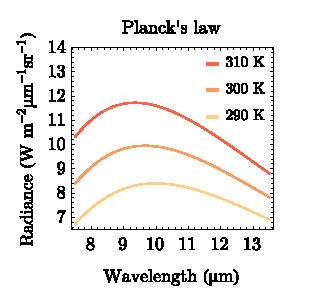
\includegraphics[scale=1]{pics/Chapter_01/PlancksLaw.eps}
		\vspace{-0.1cm}
		\caption{Radiation of black body described by Planck's law}
		\label{fig:BBradiation}
	\end{subfigure}
	\hspace{1em}
	\begin{subfigure}[t]{.3\linewidth}
		\centering
		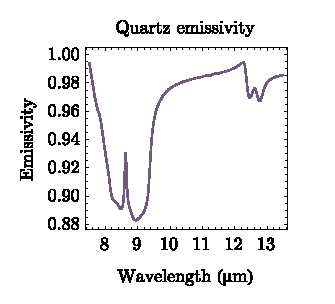
\includegraphics[scale=1]{pics/Chapter_01/QuartzSpectrum.eps}
		\vspace{-0.1cm}
		\caption{Quartz spectral emissivity}
		\label{fig:QuartzEmissivity}
	\end{subfigure}
	\hspace{1em}
	\begin{subfigure}[t]{.3\linewidth}
		\centering
		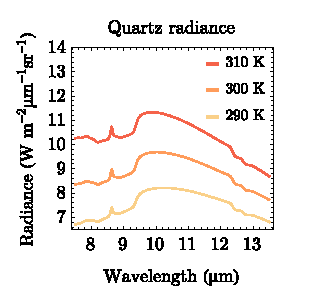
\includegraphics[scale=1]{pics/Chapter_01/QuartzRadiance.eps}
		\vspace{-0.1cm}
		\caption{Radiance of quartz}
		\label{fig:QuartzRadiance}
	\end{subfigure}
	\vspace{1.5 em}
	\caption{Principles of radiation of real surfaces.}
\end{figure}


\subsubsection*{Wien's displacement law}
The peak of black body radiation at wavelength $\lambda_{max}$ is described by Wien's displacement law \cite{H11}:
$$ \lambda_{max} = \frac{b}{T},$$
where $b$ is Wien's displacement constant ($2.8977721\,\SI{}{m}\,\SI{}{K}$). As was mentioned before, the temperature of the most of the natural and artificial surfaces observed by airborne remote sensing ranges in 270 – 330 K. According to the Wien's displacement law, the peak of emitted radiation varies roughly from $8.8\,\SI{}{\micro\meter}$ to $10.7\,\SI{}{\micro\meter}$. This range is in coincidence with the atmospheric window situated between $8\,\SI{}{\micro\meter}$ to $13\,\SI{}{\micro\meter}$. The atmospheric transmittance in this atmospheric window is very high and thus it is relevant for acquisition of remotely sensed thermal data.

\subsubsection*{Kirchhoff's law of thermal radiation}
Emitting and absorbing properties of an object at local thermodynamic equilibrium surrounded by isothermal environment are tied up by Kirchhoff's law of thermal radiation \cite{K60}. It states that object's surface absorptivity $\alpha(\lambda)$ at a given wavelength equals to object surface emissivity $\varepsilon(\lambda)$ at the same wavelength:
$$ \alpha(\lambda) = \varepsilon(\lambda). $$
Energy conservation implies that energy incident to the object surface can be reflected, transmitted or absorbed. Considering the fractions of incident energy the following equation holds:
$$ 1 = \rho(\lambda) + \tau(\lambda) + \alpha(\lambda), $$
where $\rho(\lambda)$ is objects surface spectral reflectivity, $\tau(\lambda)$ is object surface spectral transmissivity and $\alpha(\lambda)$ is object surface spectral absorptivity. Applying Kirchhoff's law to opaque material ($\tau(\lambda) = 0$) results in following equation:
$$ 1 = \rho(\lambda) + \varepsilon(\lambda) \quad \Rightarrow \quad \rho(\lambda) = 1 - \varepsilon(\lambda).$$

All mentioned principles in this section will be further used in explanation of properties of airborne thermal hyperspectral data and its processing.

	\cleardoublepage
	\pagestyle{mystyle}
\chapter{Airborne Thermal Hyperspectral Data Properties}
\label{chap:Data}

This chapter provides insights into technical parameters of Thermal Airborne Spectrographic Imager (TASI) and processing chain of image data acquired by this sensor. Knowledge of the instrument parameters and processing chain gives important overview of the image data properties and their components. The result of the processing chain described in this chapter is georeferenced image data containing land-leaving radiance. Such an image data form input for further processing. 
Let us note that this chapter omits naming physical quantities dependent on wavelength as ``spectral'' for the sake of clarity. However, all quantities remain wavelength dependent.

\section{Instrument Technical Specifications}

The TASI sensor is developed by Itres Ltd. (Calgary, Canada) and is one of the very few commercially available pushbroom hyperspectral TIR sensors equipped with mercury cadmium telluride array. Each of its 600 across-track imaging pixels contains 32 bands all of which are in the TIR region. Bands are situated in the 8 to $\SI{11.5}{\micro\meter}$ region and have a $\mathrm{FWHM} \approx \SI{0.11}{\micro\meter}$ with $\mathrm{NE\Delta T} \approx 0.1\,\mathrm{K}$. The response functions of the TASI sensor are described by the Gaussian functions as depicted in Figure \ref{fig:ResponseFunctions}. 

The shape of response functions implies that any quantity observed by TASI sensor is of finite spectral-bandwidth. Quantities needs to be transformed to band-effective quantities in order to relate them with certain wavelength. The band-effective quantities are obtained by using weighted average:
%Thus quantities measured by sensor are transformed to band-effective quantities using weighted average:
\begin{equation}
	X_i = \frac{\int_{\lambda_1}^{\lambda_2} r_i(\lambda) X(\lambda) \,\mathrm{d}\lambda}{\int_{\lambda_1}^{\lambda_2} r_i(\lambda)\,\mathrm{d}\lambda},
	\label{eq:weightedAverage}
\end{equation}
where $r_i(\lambda)$ is response function of band $i$, $\lambda_1$ and $\lambda_2$ are lower and upper boundaries of band $i$ and $X$ can be substituted by any quantity. In Figure \ref{fig:QuartzByTASI} is illustrated radiance of quartz (solid line) and band-effective values of radiance measured by the TASI sensor (red dots). Sensor of this type is available at Global Change Research Institute CAS (Brno, Czech Republic) and it is a part of Flying Laboratory of Imaging Systems (FLIS) \cite{HF14}.

\begin{figure}[thb]
	\centering
	\vspace{1em}
	\begin{subfigure}[t]{.5\linewidth}
		\centering
		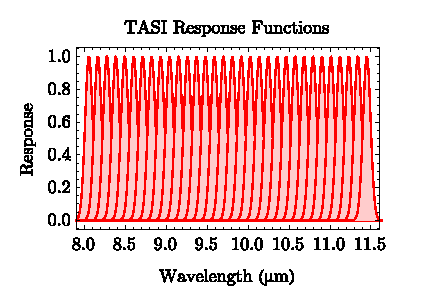
\includegraphics[scale=1]{pics/Chapter_02/TASIResponseFunctions.eps}
		\caption{Response functions of TASI sensor}
		\label{fig:ResponseFunctions}
	\end{subfigure}
	\hspace{2em}
	\begin{subfigure}[t]{.4\linewidth}
		\centering
		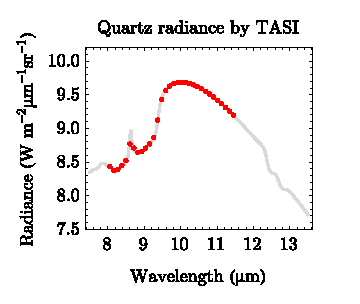
\includegraphics[scale=1]{pics/Chapter_02/QuartzByTASI.eps}
		\caption{Radiance of quartz at 300 K measured by TASI sensor}		
		\label{fig:QuartzByTASI}
	\end{subfigure}
	\vspace{1.5 em}
	\caption{TASI response functions.}
\end{figure}

\section{Image data pre-processing}

The main objective of image data pre-processing is transformation of acquired raw image data into the georeferenced radiance at-surface level. It is accomplished by three major steps: radiometric calibration, atmospheric corrections and geometric pre-processing. Radiometric calibration converts digital numbers (DN) into values of radiance at-sensor level. Atmospheric corrections compensates the influence of intervening atmosphere and produces land-leaving radiance. Finally, the geometric pre-processing compensates for image data distortions caused by aircraft movement and register image data into coordinate system.

Supportive field measurements of thermal radiance, temperature, emissivity and atmospheric parameters offers valuable data for calibration and validation purposes. Especially in cases of airborne image data for scientific purposes the high quality is strongly demanding. Thus it is necessary to perform supportive measurements in order to achieve precise results and determine the data quality.

It is important to emphasize, that currently does not exist any definitive standard pre-processing chain. It is caused mainly by huge number of sensors with various technical parameters and their different applications. Sensors usually have tailored pre-processing chains, which is the case of TASI sensor as well. Certain parts of processing chain are maintained by commercial tools. However, there are still parts of processing chain, which needs to be done by in-house tools. In Figure \ref{fig:ProcessingChain} is illustrated processing chain used in Global Change Research Institute CAS (Brno, Czech Republic) to pre-process image data acquired by TASI sensor. Individual parts of the diagram will be discussed in the following text.

\begin{figure}[thb]
	\centering
	\vspace{0.7 em}
	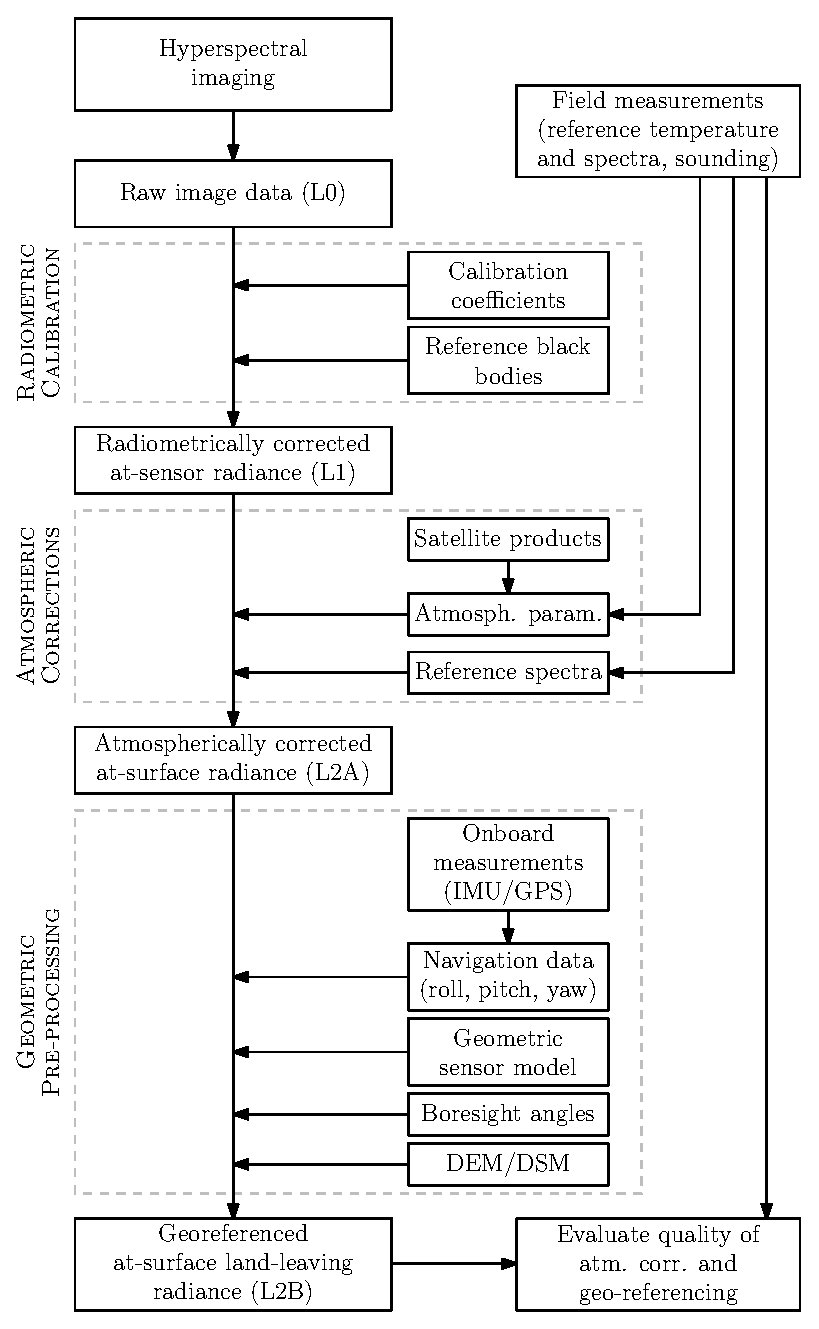
\includegraphics[scale=1]{pics/Chapter_02/Fig_2_3.eps}
	\label{fig:ProcessingChain}
	\vspace{2 em}
	\caption{Processing chain applied to image data acquired by TASI sensor.}
	\label{fig:ProcessingChain}
	\vspace{0.7 em}
\end{figure}

% show how are data modified by using different corrections -> three plots

\subsection{Radiometric Calibration}

Thermal radiation incident upon the sensor array originates from many additive components (e.g. observed scene, instrument enclosure, intervening atmosphere and others). Incident thermal radiation produces electrical signal, which is proportional to radiant intensity. Electrical signal is then amplified and converted into voltage and subsequently into DN values. Radiometric calibration consists of separating signal from viewed scene and converting it into physical units of radiance. Atmosphere influence is not accounted in this process and thus after radiometric calibration one gets radiance at-sensor level.

The relationship between DN and at-sensor radiance $L_\mathrm{m}$ is following:
$$ \mathrm{DN} = a + b L_\mathrm{m}, $$
where $a$ and $b$ are calibration coefficients. The calibration coefficient $a$, also known as offset, represents radiation originating from instrument enclosure, sensor dark current and electronic offset. The calibration coefficient $b$, also called gain, determines sensor radiant sensitivity. Calibration coefficients are determined by imaging a set of reference black bodies of known temperature and emissivity. In this context, the term black body is ment to be a surface with emissivity very close to unity. These coefficients are usually determined applying one of two methods: 1) imaging two black bodies at different temperature directly before imaging, or 2) combining black body image data from laboratory and black body image data acquired before imaging.

In the first case are usually used two black bodies of different temperatures. Temperatures of these black bodies enclose temperatures expected to occur in the scene. Let us consider the radiance of cold black body $L(T_\mathrm{C})$ and the radiance of hot blackbody $L(T_\mathrm{H})$. The calibration coefficients can be obtained from:
\begin{eqnarray*}
	a &=& \frac{\mathrm{DN}_\mathrm{H} L(T_\mathrm{C}) - \mathrm{DN}_\mathrm{C} L(T_\mathrm{H}) }{ L(T_\mathrm{C}) - L(T_\mathrm{H}) } \\
	b &=& \frac{\mathrm{DN}_\mathrm{C} - \mathrm{DN}_\mathrm{H}}{ L(T_\mathrm{C}) - L(T_\mathrm{H}) },
\end{eqnarray*}
where $\mathrm{DN}_\mathrm{C}$ and $\mathrm{DN}_\mathrm{H}$ are digital numbers measured by sensor viewing cold black body and hot black body respectively. This procedure is commonly used in case of other instruments for measuring thermal radiation, such as $\mathrm{\mu}$FTIR \ref{HK96}.

The determination of calibration coefficients in the second case assumes that gain calibration coefficient $b$ does not change under different conditions. Thus, it is sufficient to perform series of black body measurements at different temperatures in order to determine gain calibration coefficient $b$. These measurements can be performed in the laboratory once per season. However, offset calibration coefficient $a$ does not remain stable and changes under different conditions. Hence, it is necessary to image a black body at known temperature directly before acquisition to account for variability of this coefficient.

%The determination of calibration coefficients in the second case is based on the assumption of invariant gain calibration coefficient $b$ and variable offset calibration coefficient $a$ in different conditions. This implies that gain calibration coefficient $b$ is determined in laboratory by imaging reference black bodies of different temperatures and offset calibration coefficient $a$ is determined by imaging reference black body of known temperature before acquisition of data from scene.

Again, it is important to emphasize that all quantities and both calibration coefficients are wavelength dependent. Spectral calibrations are part of the radiometric calibrations. In the laboratory are determined band centers of every pixel using laser at different wavelengths. Determined positions does not change over time significantly. However, the spectral shift occurs under different conditions and thus it needs to be determined for every scene. Spectral shift estimation is usually based on the spectral features of the atmosphere or certain materials.
% TODO: upresnit jednou vetou odhad spectral shiftu

In case of TASI sensor are used commercial softwares delivered by Itres company (Calgary, Canada). SparCal software \cite{software:SparCal} is used to determine all parameters necessary for radiometric calibrations from laboratory measurements. RCX software \cite{software:RCX} is used for additional  estimation of calibration parameters and for processing raw image data. Both softwares are tailored for the TASI sensor. The resulting image data are made of radiance at-sensor level $L_\mathrm{m}$.

\subsection{Atmospheric Corrections}

Radiometric calibrations deliver image data containing radiation from the surface, attenuated by atmosphere, plus radiation from the atmosphere along the line of sight. Thus the measured radiance at-sensor level ($L_\mathrm{m}$) consists mainly of radiance emitted from the land surface, downwelling atmospheric radiance reflected by the surface ($L^\downarrow_\mathrm{atm}$) and the atmospheric upwelling radiance ($L^\uparrow_\mathrm{atm}$). The sum of all these components is expressed by a radiative transfer equation (RTE) as follows:
\begin{equation} 
\label{eq:RTE}
L_\mathrm{m} = \tau \varepsilon B(T_\mathrm{s}) + \tau (1 - \varepsilon) L^\downarrow_\mathrm{atm} + L^\uparrow_\mathrm{atm},
\end{equation}
where $B(T_\mathrm{s})$ is radiance of the surface at temperature $T_\mathrm{s}$ according to the Planck's law, $\varepsilon$ is the surface's emissivity and $\tau$ is atmospheric transmittance. It is important to emphasize that all elements in the equation are wavelength dependent but notation for this is omitted for the sake of clarity. Since sensors are of finite bandwidth, quantities in (\ref{eq:RTE}) are replaced by band-effective equivalents according to the equation (\ref{eq:weightedAverage}). Moreover, RTE can be used under the assumption of cloud-free atmosphere under local thermodynamic equilibrium. The meaning of the RTE is illustrated in the Figure \ref{fig:FigRTE}, where $\rho$ is reflectivity. Kirchhoff's law of thermal radiation implies that reflectivity $\rho$ can be rewritten as $(1 - \varepsilon)$ for opaque materials.

\begin{figure}[htbp]
	\centering
	\vspace{1em}
	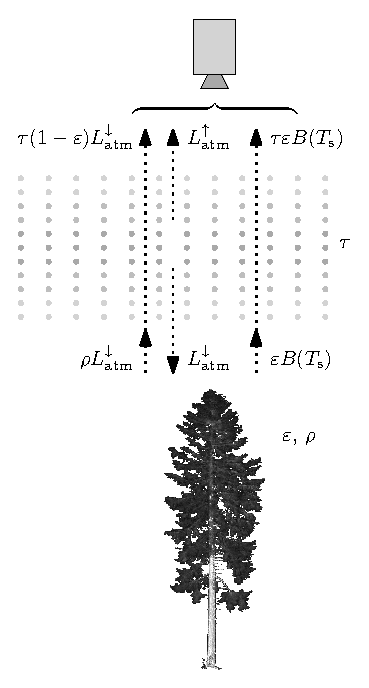
\includegraphics{pics/Chapter_02/Fig_3_2.eps}
	\vspace{1.5 em}
	\caption{The radiance incident to the sensor in the thermal region originates mainly from three sources: 1) radiance $\tau\varepsilon B(T_s)$ emitted by object; 2) reflected downwelling atmospheric radiance $\tau(1-\varepsilon)L_\mathrm{atm}^\downarrow$; 3) upwelling atmospheric radiance $L_{atm}^\uparrow$ emitted by atmosphere itself.}
	\label{fig:FigRTE}
\end{figure}

The goal of the atmospheric corrections is to determine atmospheric transmittance, downwelling and upwelling atmospheric radiance and compensate for them. The quantification of these quantities are usually based on radiative transfer models of the atmosphere. For this purpose is usually used MODerate resolution atmospheric TRANsmission (MODTRAN) model \cite{BG06}. MODTRAN simulates atmospheric parameters such as atmospheric transmittance, downwelling and upwelling atmospheric radiance based on input parameters such as vertical profiles of water vapour content and temperature, CO$_2$ concentration, the choice of model atmosphere (if measured profiles are not available) and many others. In general, input parameters can be obtained in two ways: 1) by in-situ measurements; 2) by satellite-based products.

The most common in-situ measurement is radio sounding. Radiosonde is launched during the overflight and it is used to measure vertical temperature and water vapour profile of the atmosphere. Other in-situ instruments can be used as well, for example sun-photometer for obtaining water vapor content or different radiometers for measuring sky or surface radiance. Other source of water vapour and temperature profile is satellite-based products acquired close to the time of aircraft overflight. The most common is MOD07\_L2 product \cite{B11} generated by Moderate Resolution Imaging Spectroradiometer (MODIS) instrument. Illustration of the transmittance, downwelling and upwelling atmospheric radiance generated by MODTRAN using MOD07\_L2 products as input are depicted in Figure \ref{fig:AtmParams}.

\begin{figure}[htb]
	\centering
	\vspace{1em}
	\begin{subfigure}[t]{.3\linewidth}
		\centering
		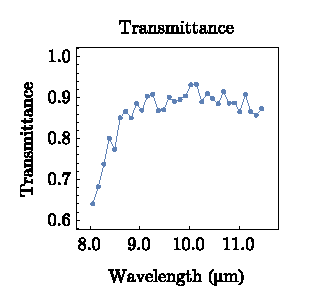
\includegraphics[scale=1]{pics/Chapter_02/Transmittance.eps}
		\vspace{-0.4cm}
		%\caption{Atmospheric transmittance}
		\caption{}
	\end{subfigure}
	\hspace{1em}
	\begin{subfigure}[t]{.3\linewidth}
		\centering
		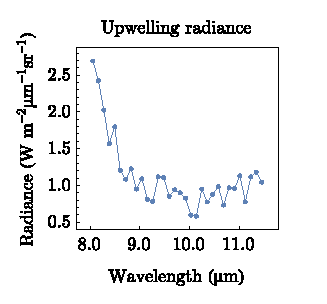
\includegraphics[scale=1]{pics/Chapter_02/Upwelling.eps}
		\vspace{-0.4cm}
		%\caption{Upwelling atmospheric radiance}
		\caption{}
	\end{subfigure}
	\hspace{1em}
	\begin{subfigure}[t]{.3\linewidth}
		\centering
		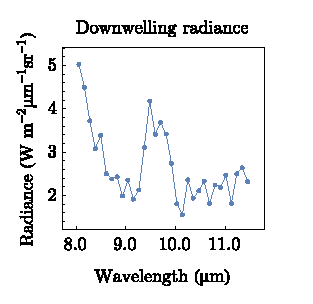
\includegraphics[scale=1]{pics/Chapter_02/Downwelling.eps}
		\vspace{-0.4cm}
		%\caption{Downwelling atmospheric radiance}
		\caption{}
	\end{subfigure}
	\vspace{1.5 em}
	\caption{Example of atmospheric parameters used for atmospheric correction of TASI image data acquired at altitude of \SI{2000}{\meter} during summer season.}
	\label{fig:AtmParams}
\end{figure}

In case of thermal hyperspectral images, various algorithms for estimating atmospheric effects based just on the image data itself were developed. Usually it is applied to one of the following: In-Scene Atmospheric Corrections (ISAC) introduced by Young et al. \cite{Y02} and Autonomous Atmospheric Compensation (AAC) introduced by Gu et al. \cite{GG00}. The advantage of using one of these algorithms is that no supporting data are necessary. The drawback of these methods remains in estimation of just atmospheric transmittance and upwelling atmospheric radiance.

Once all the atmospheric parameters are determined, it remains to compensate for them. Compensating for atmospheric transmittance and upwelling atmospheric radiance lead to land-leaving radiance:
\begin{equation}
\label{eq:landleavingRadiance}
L_\mathrm{LL} = \varepsilon B(T_\mathrm{s}) + (1 - \varepsilon) L^\downarrow_\mathrm{atm}.
\end{equation}
The downwelling atmospheric radiance is not possible to separate without knowledge of emissivity. Hence, image data after atmospheric corrections are made of land-leaving radiance $L_\mathrm{LL}$. Compensation for downwelling atmospheric radiance is part of the temperature and emissivity separation described in Chapter \ref{chap:TES}.

Atmospheric corrections for TASI sensor, as part of processing chain, are not performed by commercial products. However, there exists commercial tools that allows complex solution for atmospheric corrections. An example of such a tool is ATCOR \cite{RS02} which is based on look-up tables generated by MODTRAN and takes into account terrain topography and sensor parameters. It offers basic temperature and emissivity separation algorithms as well. Apart of mentioned solution, atmospheric corrections rely on extracting data from in-situ measurements or satellite products, running radiative transfer models and applying derived atmospheric parameter on image data. Alternatively, algorithms for atmospheric parameters estimation from image data can be implemented. In both cases, atmospheric corrections involve creating in-house tools.

\begin{figure}[htb]
	\centering
	\vspace{1em}
	\begin{subfigure}[t]{.3\linewidth}
		\centering
		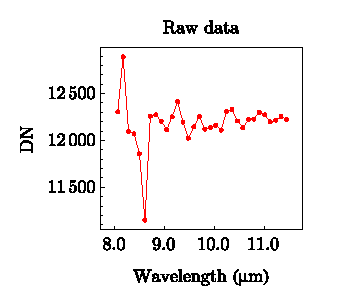
\includegraphics[scale=1]{pics/Chapter_02/calibration-1-DN.eps}
		\vspace{-0.4cm}
		%\caption{Raw image of quartz in DN values}
		\caption{}
	\end{subfigure}
	\hspace{1em}
	\begin{subfigure}[t]{.3\linewidth}
		\centering
		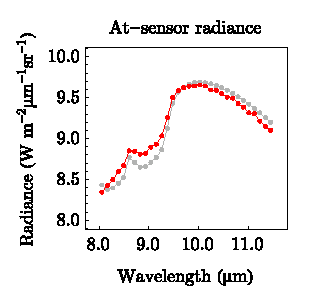
\includegraphics[scale=1]{pics/Chapter_02/calibration-2-Lm.eps}
		\vspace{-0.4cm}
		%\caption{At-sensor radiance of quartz}
		\caption{}
	\end{subfigure}
	\hspace{1em}
	\begin{subfigure}[t]{.3\linewidth}
		\centering
		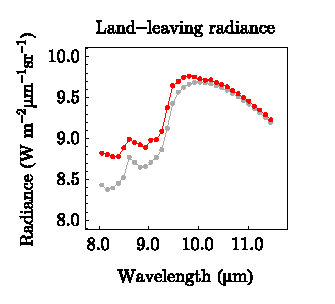
\includegraphics[scale=1]{pics/Chapter_02/calibration-3-Lll.eps}
		\vspace{-0.4cm}
		%\caption{Land-leaving radiance of quartz.}
		\caption{}
	\end{subfigure}
	\vspace{1.5 em}
	\caption{Example of data at various processing stages. Data simulates quartz at \SI{300}{\kelvin} as would be acquired by TASI sensor at altitude of \SI{2000}{\meter} under summer mid-latitude atmosphere. Case (a) shows raw data, case (b) shows data after radiometric calibration (in red) and case (c) shows data after corrections of atmospheric transmissivity and upwelling atmospheric radiance (in red). In cases (b) and (c) are shown pure quartz radiance in gray.}
	\label{fig:RadAtmCorOfQuartz}
\end{figure}

\subsection{Geometric Pre-processing}

Acquired image data are distorted during its acquisition and geometric pre-processing is accounting for all factors causing these distortions. During geometric pre-processing are taken into account aircraft motion, terrain variations and geometric sensor model in order to register image data into reference frame.

Ancillary data about aircraft position and movement, terrain structure and geometric sensor model are necessary. Aircraft needs to be equipped with IMU/GNSS systems for recording aircraft position (longitude, latitude and altitude) and orientation (roll, pitch and heading angles). Terrain structure is obtained form Digital Surface Model (DSM) or Digital Elevation Model (DEM). These data are derived from aerial laser scanning or from stereo images. Aerial laser scanning can be performed either simultaneously with image data acquisition or separately. Other sources of DEM/DSM are national services or satellite products (e.g. ASTER product AST14DEM). Geometric sensor model is usually delivered by sensor manufacturer.

The process applied on image data during geometric pre-processing is called geo-othoreferencing. It consists of two successive steps: direct image data geocoding and resampling. Direct image data geocoding consists of geometric corrections and orthogonalization of the image data. These are further resampled into regular grid of the reference frame with the desired coordinate system (e.g. Universal Transverse Mercator coordinate system). Image data are resampled into desired spatial resolution applying nearest neighbor, bilinear or cubic interpolation. For the scientific purposes is commonly used nearest neighbor interpolation since it preserves spectral information and does not combine spectra from surrounding pixels.

Geometric pre-processing of the image data acquired by TASI sensor are performed by GeoCor software \cite{software:GCSS} delivered by Itres company (Calgary, Canada). Importance of image data geometric pre-processing is illustrated in the Figure \ref{fig:Georeferencing}. 

\begin{figure}[thb]
	\centering
	\vspace{1em}
	\begin{subfigure}[t]{.38\linewidth}
		\centering
		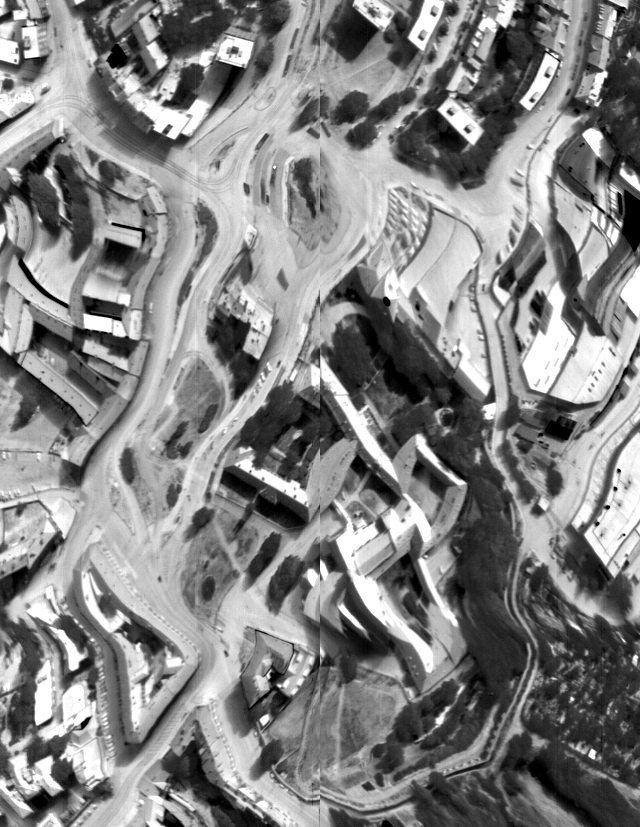
\includegraphics[scale=0.24]{pics/Chapter_02/TASIcalibrated.png}
		\caption{Distorted image data}
		\label{fig:ResponseFunctions}
	\end{subfigure}
	\hspace{2em}
	\begin{subfigure}[t]{.52\linewidth}
		\centering
		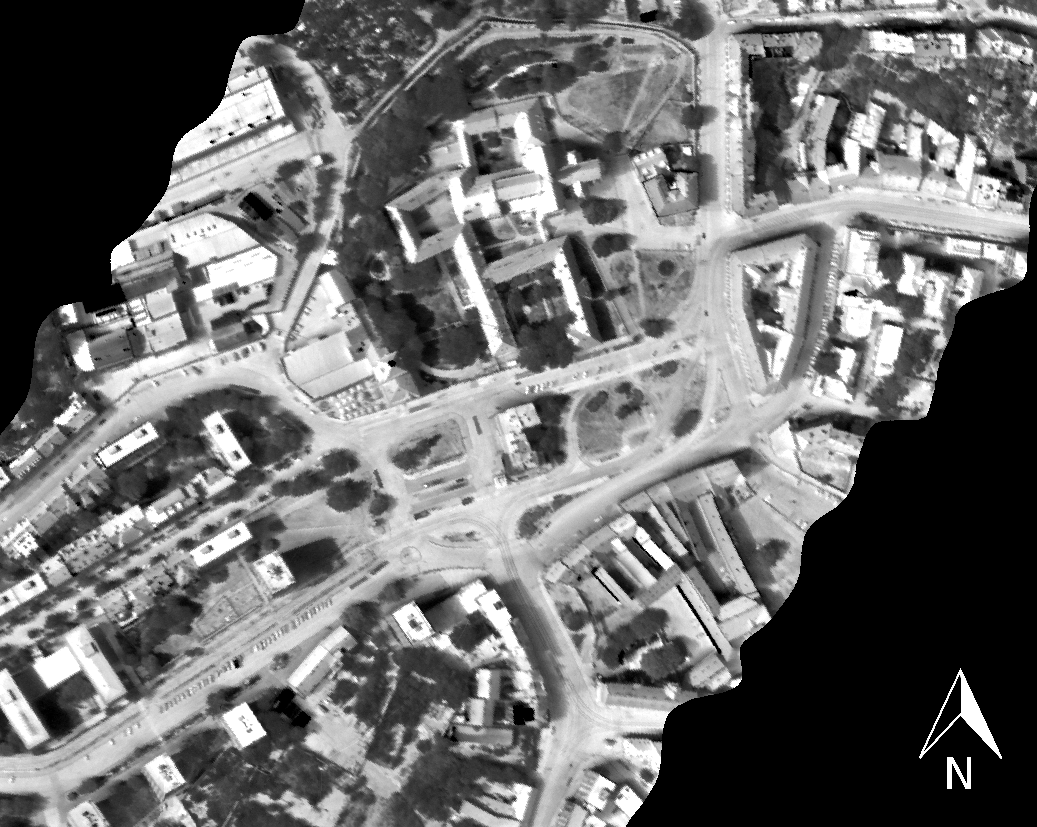
\includegraphics[scale=1]{pics/Chapter_02/TASIgeoreferencedcut.png}
		\caption{Georeferenced image data}		
		\label{fig:QuartzByTASI}
	\end{subfigure}
	\vspace{1.5 em}
	\caption{Illustration of land-leaving radiance image data before and after geometric pre-processing.}
	\label{fig:Georeferencing}
\end{figure}




	\cleardoublepage
	\pagestyle{mystyle}
\chapter{Temperature and Emissivity Separation}
\label{chap:TES}

Pre-processed thermal image data provide valuable information about the properties of the observed surfaces, most importantly their temperature and emissivity. But in order to determine temperature and emissivity from observed radiance one must solve system of RTEs. Data from multispectral and hyperspectral TIR sensors offer the opportunity to derive both the temperature as well as an emissivity spectrum, which can be used to characterize the material composition of surfaces. However, observing radiance in $N$ bands yields $N$ RTEs but $N+1$ unknowns ($N$ emissivities plus temperature), which results in the underdetermined system of equations. The estimation of temperature and emissivity from such a system of equations is usually addressed as \textit{temperature-emissivity separation}. This chapter describes several approaches for separating temperature and emissivity. It firstly introduces few commonly used ones and then focuses on the most popular approach called Temperature and emissivity separation algorithm (TES). Last part of this chapter focuses on enhancing the accuracy and precision of the products generated by the TES algorithm. The main improvement is accomplished by replacing one of the TES modules with a newly designed one that takes advantage of a relationship between brightness temperature and emissivity. The improved TES algorithm is called Optimized Smoothing for Temperature Emissivity Separation (OSTES).

\section{Available approaches}

Many approaches have been developed to overcome the problem of having an underdetermined system of RTEs \cite{LT13}. Methods used to overcome the problem of underdetermined system of RTEs are usually based on adding empirical or semiempricial constraints. 

Algorithms for temperature and emissivity estimation depend on sensor architecture and acquisition context. Some algorithms require knowledge of Normalized Difference Vegetation Index (NDVI) \cite{SR00}, surface type \cite{SW98} or even emissivity \cite{JC09}. Others are based on multitemporal \cite{W08} or multiangle \cite{SS07} acquisition. There are only a small number of algorithms for simultaneous temperature and emissivity retrievals from a single scene without ancillary surface information, that are robust enough to be applicable to data acquired by multispectral or hyperspectral sensors. The most common are: grey body emissivity method \cite{BP96}, linear emissivity constraint temperature emissivity separation method \cite{WW11}, spectral smoothing \cite{B08} and the TES algorithm \cite{GR98}. Principles of last four mentioned methods are described in the following text. The most attention is paid to the TES algorithm, as it is the most popular and it is widely applied to many sensors.

\subsection*{Gray body emissivity method}

Barducci and Pippi \cite{BP96} proposed algorithm, which is based on assumption of flat spectral emissivity beyond $\SI{10}{\micro\meter}$. To solve the system of RTEs it is enough to find at least two spectral bands with the same emissivity. This can be achieved in case of airborne thermal hyperspectral data. Drawback of this method is its sensitivity to instrument noise.

\subsection*{Linear emissivity constraint temperature emissivity separation method}

As Wang et al. \cite{WW11} describe, this method is based on idea of substituting spectral emissivity with piecewise linear function. The emissivity spectrum is divided into segments, in which spectral emissivities are assumed to be linearly dependent on wavelength. Thus, it is necessary for every segment to estimate gain and offset. It implies that the number of spectral bands has to be equal or greater than number of unknowns resulting from segmentation to piecewise linear functions.

\subsection*{Spectral smoothing}

Spectral smoothing algorithm, also known as ARTEMISS (Automatic Retrieval of Temperature and EMIssivity using Spectral Smoothness), was reported by Borel at \cite{B98} and \cite{B08}. Algorithm is based on the assumption that spectra of solids are much more smoother than spectra of gases. Thus by smoothing spectra one removes spectral features introduced by atmosphere and obtains spectral emissivity. Moreover, current implementation described in \cite{B08} includes modified ISAC algorithm called ARTISAC, which estimates atmospheric transmissivity for further choice correct atmospheric model. Atmospheric models contains so called TUD (atmospheric Transmissivity, Upwelling and Downwelling atmospheric radiance) and are stored in look-up tables (LUT). Then temperature is varied until the spectral emissivity is the smoothest possible, where the smoothness criterion is standard deviation of measured radiance minus simulated radiance. Spectral smoothness method can be described briefly by following steps:
\begin{enumerate}
	\item estimation atmospheric transmissivity using ARTISAC algorithm
	\item determination few closest atmosphere models from TUD-LUT according to the estimated atmospheric transmissivity
	\item use these atmosphere models as input to spectral smoothness algorithm for a few pixels chosen from the image and the atmosphere model which results in smoothest emissivity in the most of the cases is chosen as the correct one
	\item use chosen atmosphere model for the whole image and estimate temperature and emissivity by applying spectral smoothing procedure
\end{enumerate}

\section*{Temperature and emissivity separation algorithm (TES)}

TES algorithm was originally developed for the Advanced Spaceborne Thermal Emission and Reflection Radiometer (ASTER) sensor \cite{GR98}. ASTER was launched in December 1999 onboard NASA's Terra platform. TES has since then found widespread use with other multispectral and hyperspectral sensors.

Several studies have discussed the implementation of TES with Airborne Hyperspectral Scanner (AHS) data \cite{SJ06, JS12}. Application of TES to data acquired by the TASI sensor is mentioned in a few studies as well \cite{WX11, PP12}. Apart from the mentioned sensors, the TES algorithm has been modified for the Digital Airborne Imaging Spectrometer (DAIS) sensor \cite{SJ02}. Concerning spaceborne sensors, the TES algorithm has also been suggested for Spinning Enhanced Visible and Infrared Imager (SEVIRI) \cite{JS14}, Moderate Resolution Imaging Spectroradiometer (MODIS) \cite{HH11} and Multispectral Thermal Imager (MTI) \cite{MB02} data processing. Moreover, the TES algorithm is being suggested for the future HyspIRI mission \cite{HH11-2}.

The TES algorithm is based on a semi-empirical relationship between spectral contrast (i.e. difference between the highest and lowest values in the emissivity spectrum) and the minimum emissivity. The algorithm consists of three modules, namely the Normalization Emissivity Module (NEM) \cite{G86}, the Ratio module and the Maximum-Minimum Difference (MMD) module \cite{M94}. The inputs of the algorithm are land-leaving radiance $L_\mathrm{LL}$ and downwelling radiance $L^{\downarrow}_\mathrm{atm}$. Let us remind the reader that land-leaving radiance is obtained from (\ref{eq:RTE}) by compensating for atmospheric transmissivity $\tau$ and atmospheric upwelling radiance $L^{\uparrow}_\mathrm{atm}$:
\begin{equation}
\label{eq:landleavingRadiance}
L_\mathrm{LL} = \varepsilon B(T_\mathrm{s}) + (1 - \varepsilon) L^\downarrow_\mathrm{atm}.
\end{equation}

The NEM module performs an iterative process for estimating temperature and emissivity, and compensating for the downwelling radiance. The output of the NEM module is an initial estimation of temperature and emissivity. Then the ratio module normalizes the emissivities obtained by the NEM module by their arithmetic mean. Thus one obtains the so called $\beta$ spectrum, which should be less sensitive to sensor noise. Finally, the maximum and minimum of the $\beta$ spectrum are found and their difference (MMD) is used in following semi-empirical relationship:
\begin{equation} 
\label{eq:MMD}
\varepsilon_\mathrm{min} = 0.994 - 0.687 \times \mathrm{MMD}^{0.737}. 
\end{equation}
Derivation of (\ref{eq:MMD}) is explained in following paragraph. Ratioing the $\beta$ spectrum back to an emissivity spectrum with knowledge of minimum emissivity results in a more precise estimation of the emissivity spectrum. The band with highest emissivity is then used for temperature estimation.

The relationship between spectral contrast and minimum emissivity, shown in (\ref{eq:MMD}), is a regression based on 86 laboratory spectra of rocks, soils, vegetation, snow and water chosen from the ASTER spectral library \cite{BH09}. This relationship is depicted in the Figure \ref{fig:EpsMinMMD}. It is important to note that (\ref{eq:MMD}) is tailored for the ASTER sensor. To apply  {TES to a} different sensor,  {the} regression of $\varepsilon_\mathrm{min}$ on MMD  {must be} refined by using sensor specific response functions. 

\begin{figure}[thb]
	\centering
	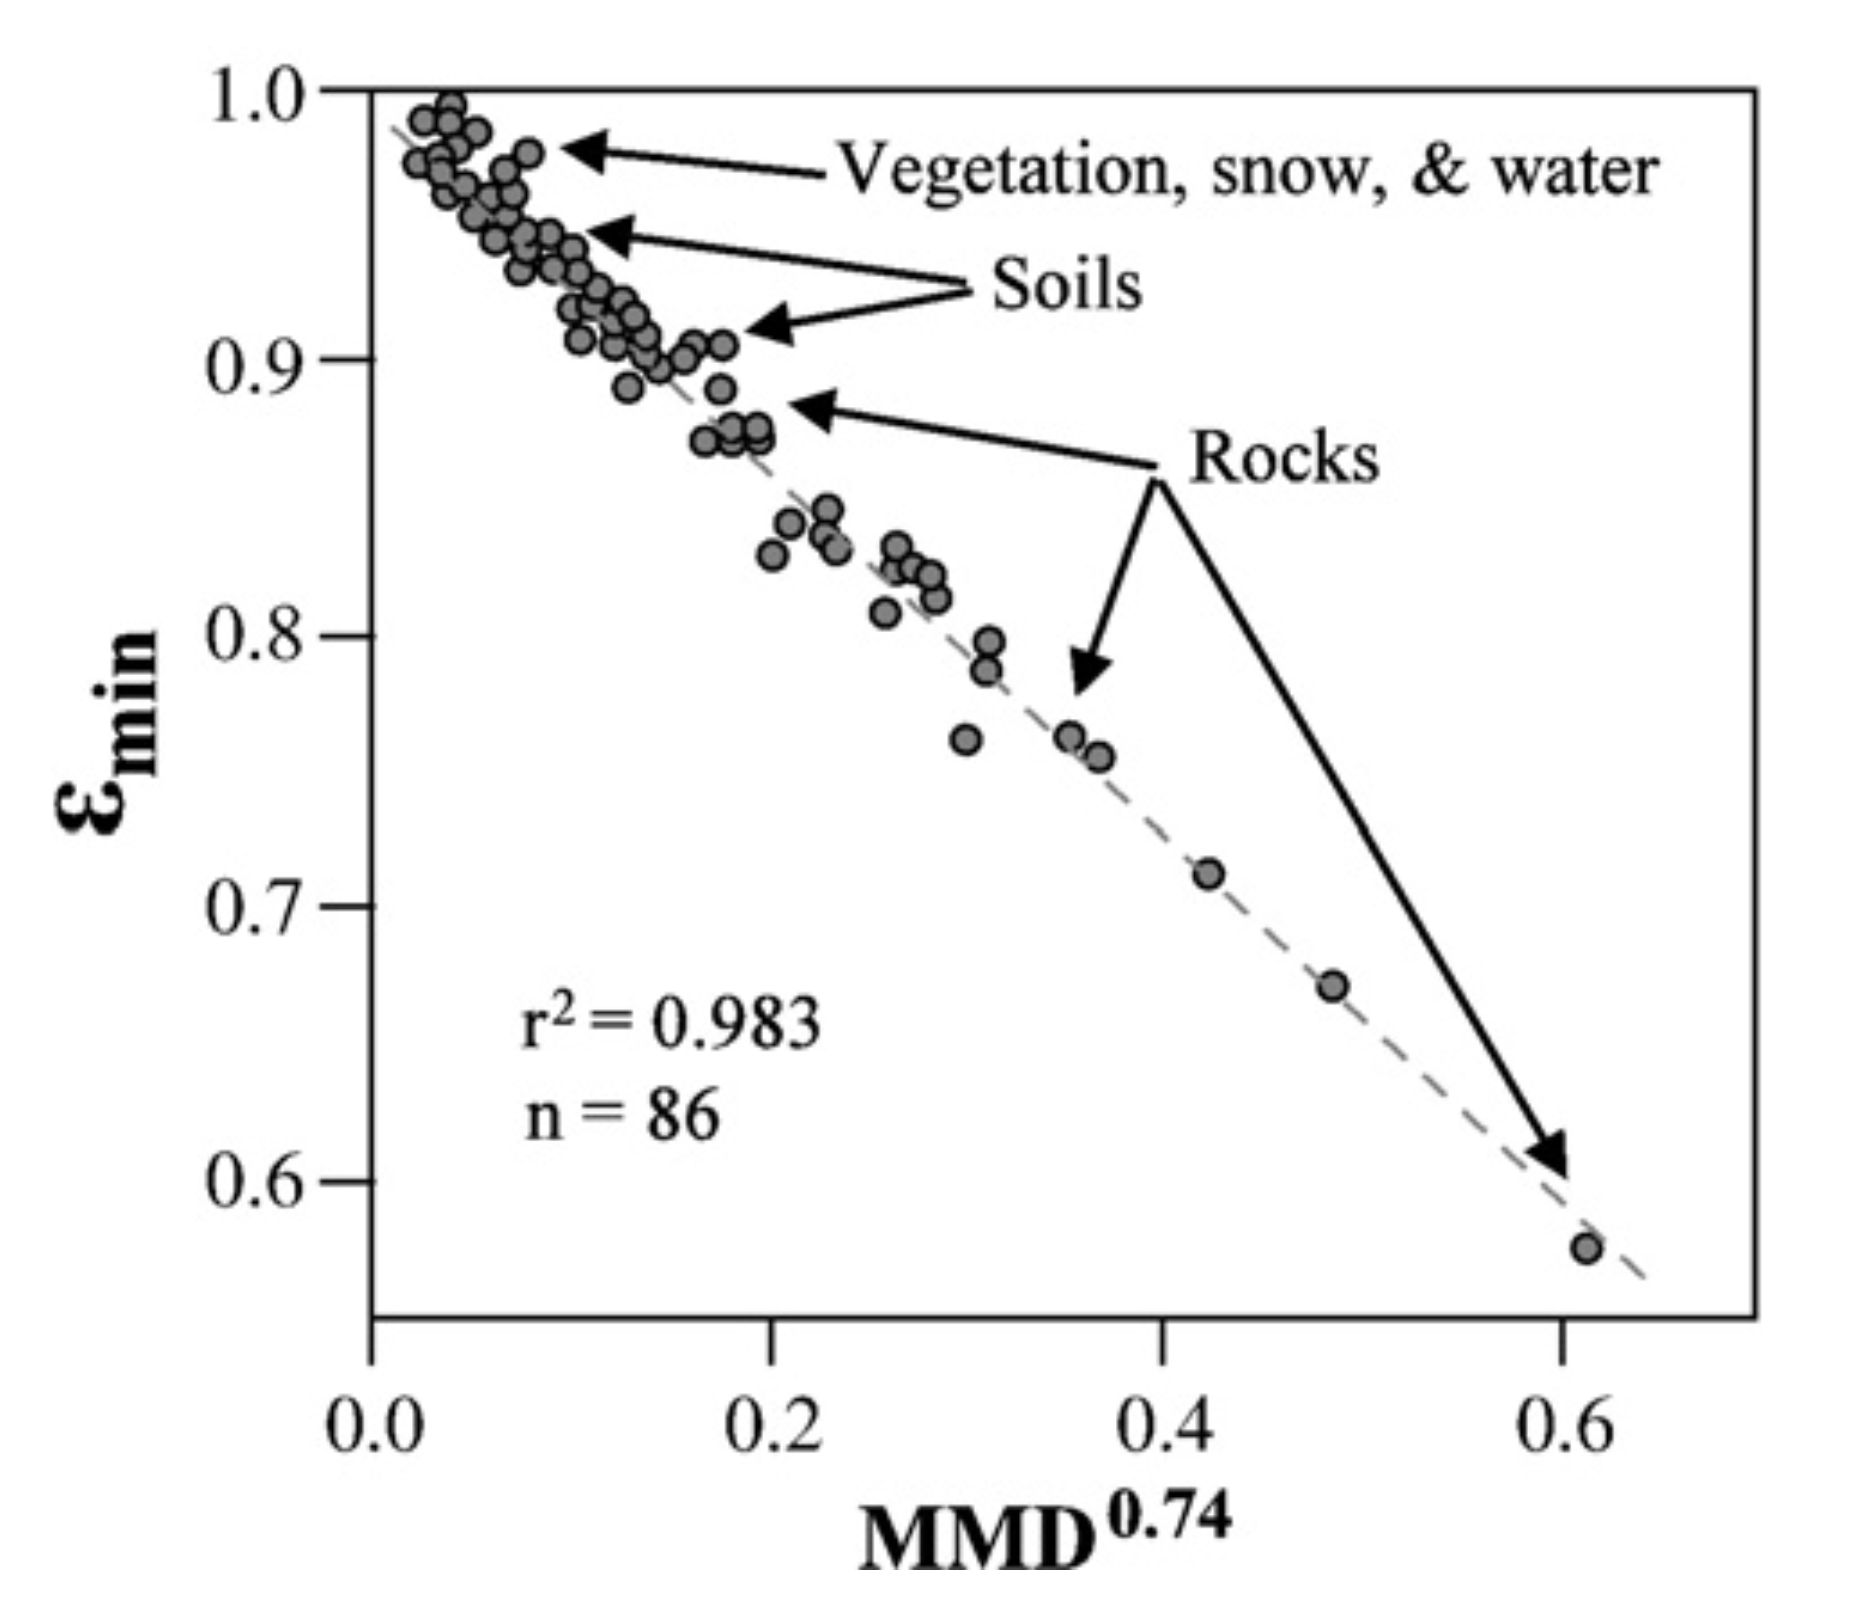
\includegraphics[scale=0.2]{pics/Chapter_03/EpsMinMMD.png}
	\vspace{1.5 em}
	\caption{Semi-empirical relationship between emissivity contrast and minimum spectral emissivity as shown in study reported by Sabol et al. \cite{SG09}.}
	\label{fig:EpsMinMMD}
\end{figure}

After ASTER was launched, \cite{GG06} and \cite{SG09} suggested to replace the power regression shown in (\ref{eq:MMD}) with linear regression. The replacement is connected with modification of the threshold for separating materials with low spectral contrast. The main advantage is elimination of artefacts in retrievals. However, the drawback is loss of accuracy in cases of materials with low spectral contrast \cite{SG09}. The TES algorithm used for generation ASTER standard products \cite{B15}, as well as its modifications for other sensors \cite{SJ06, JS12, WX11, SJ02, JS14, HH11, MB02, HH11-2}, is based on the power law regression. Thus, in this work the TES algorithm is considered to be that using the power regression.

\section{TES Algorithm Improvement}

he algorithm described below brings a new approach for the TES algorithm by replacing the NEM module with a completely new module. The new module is based on the similarity between brightness temperature spectral features and emissivity spectral features. Brightness temperature is obtained from land-leaving radiance under the assumption of emissivity $\varepsilon=1$ for every wavelength. Although land-leaving radiance includes some portion of reflected downwelling radiance, it still retains the spectral features arising from the emissivity of the surface materials, which is $0.6$ or higher for natural materials \cite{GR98}. Since the magnitude of downwelling radiance is usually much lower than the surface radiance the features contained in the brightness temperature spectra may be distorted but will not be completely hidden. The new module approximates this relation between brightness temperature $T_\mathrm{b}$ and emissivity.

\begin{figure}[thb]
	\centering
	\vspace{1em}
	\begin{subfigure}[t]{.3\linewidth}
		\centering
		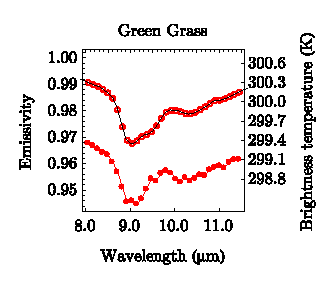
\includegraphics[scale=1]{pics/Chapter_03/GreenGrass_Emiss_vs_BrightTemp.eps}
		\vspace{-0.4cm}
		%\caption{Atmospheric transmittance}
		\caption{}
	\end{subfigure}
	\hspace{1em}
	\begin{subfigure}[t]{.3\linewidth}
		\centering
		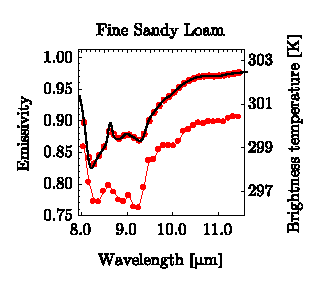
\includegraphics[scale=1]{pics/Chapter_03/FineSandyLoam_Emiss_vs_BrightTemp.eps}
		\vspace{-0.4cm}
		%\caption{Upwelling atmospheric radiance}
		\caption{}
	\end{subfigure}
	\hspace{1em}
	\begin{subfigure}[t]{.3\linewidth}
		\centering
		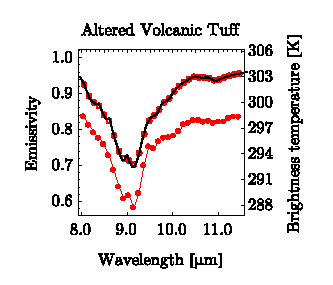
\includegraphics[scale=1]{pics/Chapter_03/AlteredVolcanicTuff_Emiss_vs_BrightTemp.eps}
		\vspace{-0.4cm}
		%\caption{Downwelling atmospheric radiance}
		\caption{}
	\end{subfigure}
	\vspace{1.5 em}
	\caption{Emissivity spectra (black solid line) of three samples chosen from ASTER spectral library \cite{BH09}. Symbols represent band-effective values of emissivity (empty symbols) and brightness temperature (full symbols) for ASTER (orange triangles), AHS (blue squares), and TASI (green dots) sensor. }
	\label{fig:emissivitySpectra_spectra}
\end{figure}

In order to demonstrate the relationship, three emissivity samples with different spectral contrasts were chosen from the ASTER spectral library, namely green grass, fine sandy loam and altered volcanic tuff. Emissivities are depicted in Fig. \ref{fig:emissivitySpectra_spectra} (solid lines) together with corresponding band-effective values for TASI sensor (empty symbols). These emissivities were applied to Plank's law at temperature $300\,\mathrm{K}$ and combined with downwelling radiance from standard mid-latitude summer atmosphere generated by MODerate resolution atmospheric TRANsmission (MODTRAN) \cite{BG06}. The resulting radiances, were transformed to band-effective quantities with respect to the ASTER, AHS and TASI response functions. Brightness temperatures for every band of each sensor were obtained by applying inverse Planck's law on sample land-leaving radiances under the assumption of $\varepsilon=1$. Fig. \ref{fig:emissivitySpectra_spectra} also includes brightness temperatures (full symbols) in order to demonstrate spectral similarity with emissivity. Fig. \ref{fig:relationship} plots emissivity against brightness temperature for chosen samples (empty symbols). These quantities clearly exhibit relationship with linear trend regardless of spectral contrast. Also displayed in Fig. \ref{fig:relationship} are lines that approximate this relationship, derived in the manner described later in the next. The algorithm description below uses band-effective values of quantities linked to $i$-th band by subscript index $i$. 

\begin{figure}[thb]
	\centering
	\vspace{1em}
	\begin{subfigure}[t]{.3\linewidth}
		\centering
		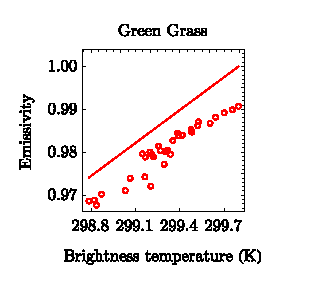
\includegraphics[scale=1]{pics/Chapter_03/GreenGrass_Emiss2BrightTemp.eps}
		\vspace{-0.4cm}
		%\caption{Atmospheric transmittance}
		\caption{}
	\end{subfigure}
	\hspace{1em}
	\begin{subfigure}[t]{.3\linewidth}
		\centering
		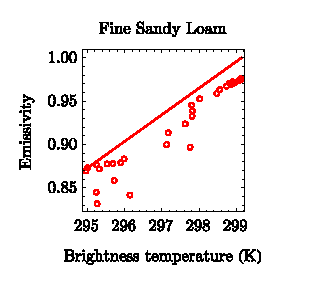
\includegraphics[scale=1]{pics/Chapter_03/FineSandyLoam_Emiss2BrightTemp.eps}
		\vspace{-0.4cm}
		%\caption{Upwelling atmospheric radiance}
		\caption{}
	\end{subfigure}
	\hspace{1em}
	\begin{subfigure}[t]{.3\linewidth}
		\centering
		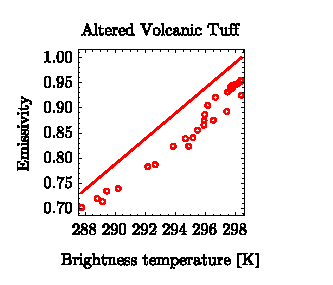
\includegraphics[scale=1]{pics/Chapter_03/AlteredVolcanicTuff_Emiss2BrightTemp.eps}
		\vspace{-0.4cm}
		%\caption{Downwelling atmospheric radiance}
		\caption{}
	\end{subfigure}
	\vspace{1.5 em}
	\caption{Symbols represents examples of the relationship between brightness temperature $T_\mathrm{b}$ and emissivity as would be observed by ASTER (orange triangles), AHS (blue squares), and TASI (green circles). Lines illustrate the approximations of the relationship between brightness temperature and emissivity for ASTER (orange dotted line), AHS (blue dashed line), and TASI (green full line) sensor. The procedure used for estimation  {of} the brightness temperature and emissivity relationship is described in text.}
\label{fig:relationship}
\end{figure}


Spectral features of brightness temperature will be further used for emissivity estimation. The dependence of emissivity $ {\varepsilon_i}$ on brightness temperature $ {T_{\mathrm{b}_i}}$ will be approximated by following equation:
\begin{equation} \varepsilon_{ {i}} =  {p} T_{\mathrm{b}_{ {i}}} +  {q}, \label{eq:relationship}\end{equation}
where $ {p}$ and $ {q}$ are empirical coefficients. These coefficients are determined by solving the system of two equations using two points, namely maximum brightness temperature coupled with emissivity equal to 1 and minimum brightness temperature coupled with lowest emissivity $\varepsilon_\mathrm{min}$:
\begin{equation}
\begin{aligned}
	1 &=  {p} \max (T_{\mathrm{b}_{ {i}}}) +  {q}, \\
	\varepsilon_\mathrm{min} &=  {p} \min (T_{\mathrm{b}_{ {i}}}) +  {q}.
\end{aligned}
\label{eq:sytemofeq}
\end{equation}
The next step is estimation of the the lowest emissivity $\varepsilon_\mathrm{min}$.

This is done by varying $\varepsilon_\mathrm{min}$ over the range  {of possible emissivities for natural materials $[0.6,1{ {]}}$}, determining corresponding coefficients $ {p}$ and $ {q}$ by solving (\ref{eq:sytemofeq}) and then approximating emissivity by (\ref{eq:relationship}) using brightness temperature for all spectral bands. The estimated emissivity is then used together with land-leaving radiance $L_\mathrm{LL}$ and downwelling radiance $L^\downarrow$ in a computation that yields spectral radiance:
\begin{equation}
	L^{\prime}_{ {i}} = \frac{L_{\mathrm{LL}_{ {i}}}-(1-\varepsilon_{ {i}})L^\downarrow_{ {i}}}{\varepsilon_{ {i}}}.
	\label{eq:lprime}
\end{equation}
The temperature in every spectral band is derived from spectral radiance $L^{\prime}$ applying inverse Plank's law. The highest one is chosen as the reference temperature $T_\mathrm{max}$. Finally, the estimated spectral radiance $L^{\prime}$ and Planck's law at the reference temperature $T_\mathrm{max}$ are normalized and compared against each other as follows:
\begin{equation}
	\sum_{ {i}} \left| \frac{B_{ {i}}(T_\mathrm{max})}{||B(T_\mathrm{max})||_1} - \frac{L^\prime_{ {i}}}{||L^\prime||_1} \right|.
\end{equation}
The value of $\varepsilon_\mathrm{min}$ is considered final if its corresponding spectral radiance $L^{\prime}$  {is the best fit to Plank's law}.

The whole process of determining $\varepsilon_\mathrm{min}$ can be understood as smoothing the spectrum by finding the optimal value of $\varepsilon_\mathrm{min}$. Pseudocode depicted in Fig. \ref{fig:FunctionCode} summarizes the above described procedure as a function \textsc{SmoothingErr}($\varepsilon_\mathrm{min},L_\mathrm{LL},L^\downarrow$) evaluating the error between Planck's law and estimated spectral radiance. This function is minimized with respect to the variable $\varepsilon_\mathrm{min}$ as follows:
\begin{equation}
\underset{\varepsilon_\mathrm{min} \in  {[0.6,1]}}{\text{arg\,min}}\:\text{\textsc{SmoothingErr}}(\varepsilon_\mathrm{min},L_\mathrm{LL},L^\downarrow).
\label{eq:costFunction}
\end{equation}

\begin{figure}[!t]
\centering
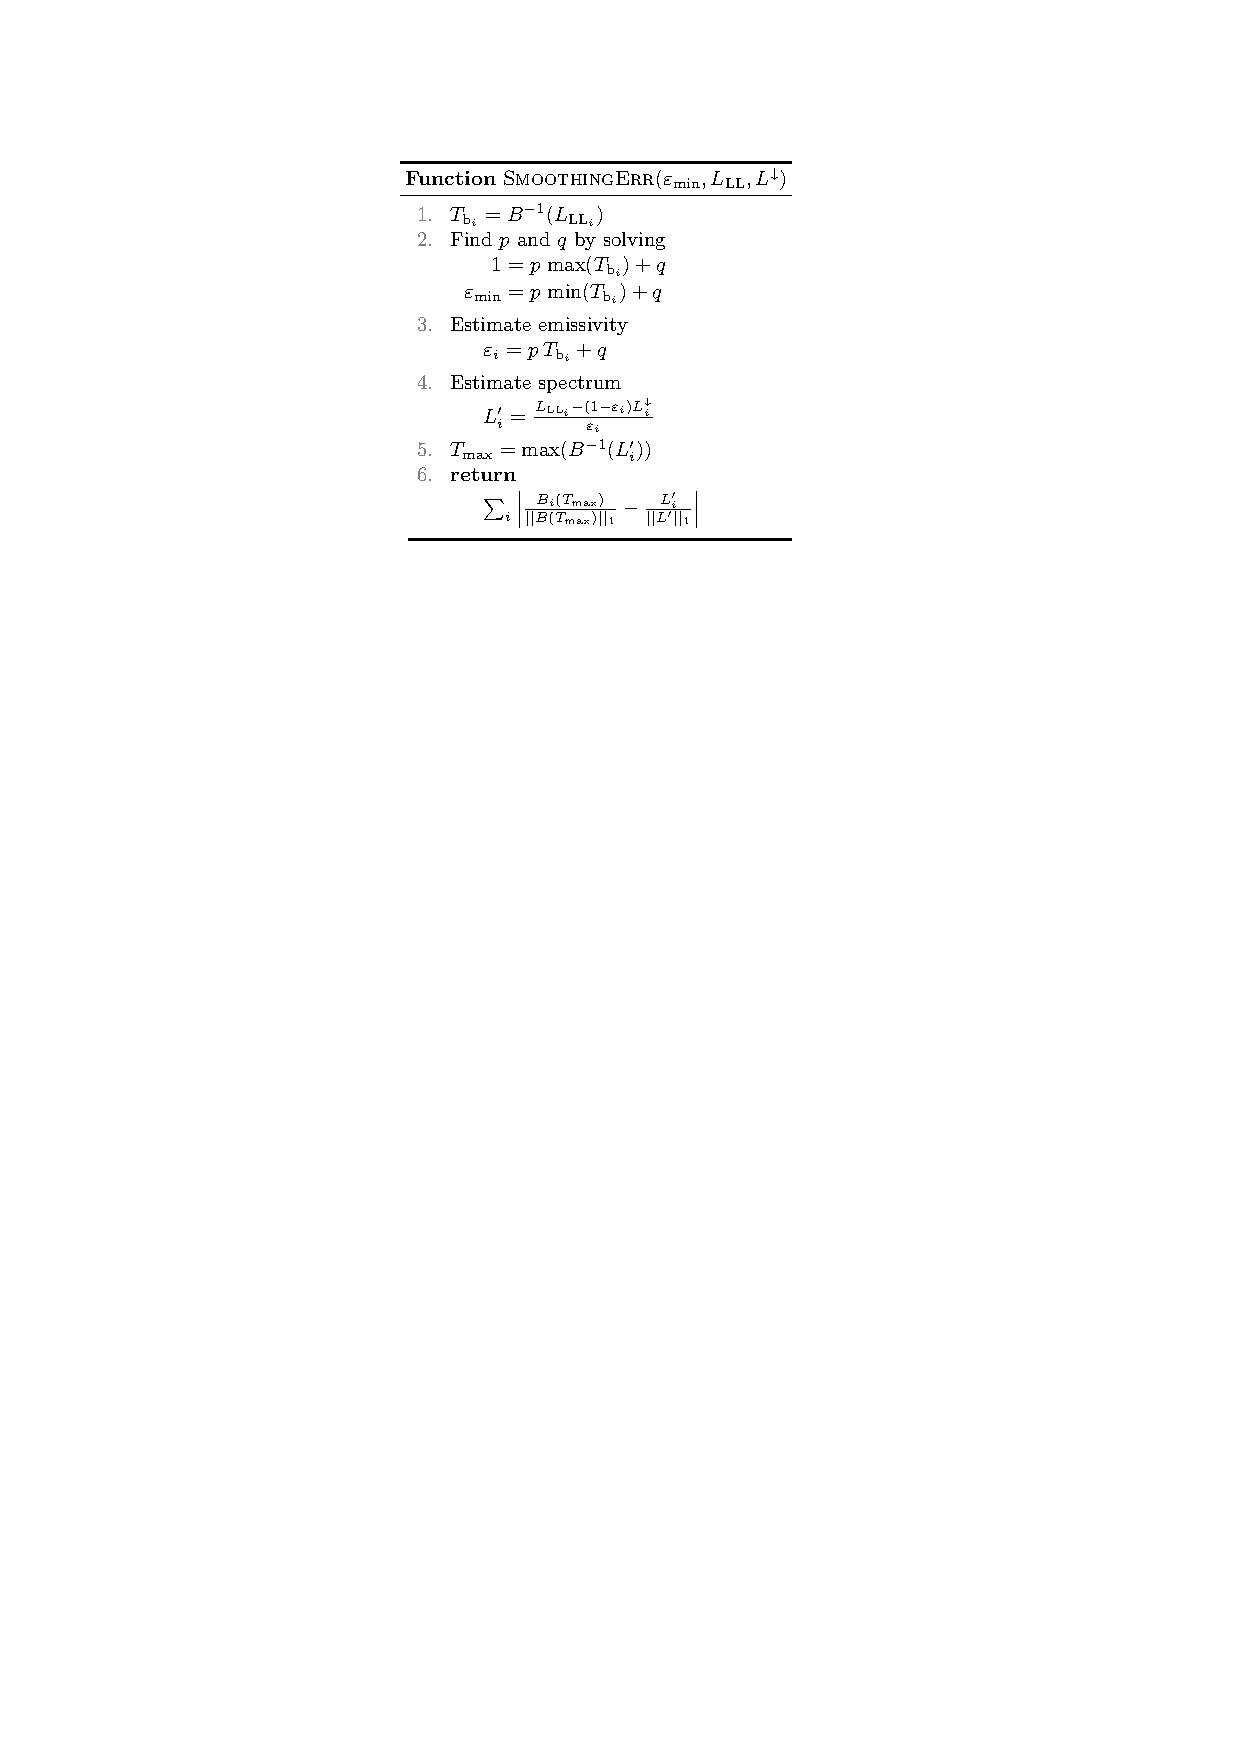
\includegraphics[width=2.2in]{pics/Chapter_03/pseudo_code.pdf}
\vspace{1.5 em}
\caption{Pseudocode of the function that is being minimized in order to estimate the value of $\varepsilon_\mathrm{min}$.}
\label{fig:FunctionCode}
\end{figure}

Continuous curves in Fig. \ref{fig:relationship} show the optimal brightness temperature and emissivity relationship approximation.  {
Let us emphasize that by applying emissivities obtained from the approximated relationship between brightness temperature and emissivity to (\ref{eq:lprime}), one gets $L^\prime$ as the best fit to Planck's law. This means that $B^{-1}(L^\prime_i)$ produces a temperature value for each band. These temperatures have minimum variability since they are derived from the best fit to Planck's law. Let us also remind the reader that maximum brightness temperature is coupled with emissivity equal to 1, which implies that it is part of the set of temperatures with smallest variability. It is important to note that maximum brightness temperature $T_\mathrm{b}$ computed from land-leaving radiance is usually smaller than surface temperature $T$ computed from surface radiance. Land-leaving radiance is smaller than surface radiance since natural materials are of emissivity higher than $0.6$ and the contribution from reflected downwelling radiance is usually much lower than surface radiance. By reason of maximum brightness temperature $T_\mathrm{b}$ being smaller than surface temperature $T$ and by being part of the set of temperatures with smallest variability, it can be concluded that maximum temperature from the set of temperatures tends to be the closest to the surface temperature $T$ and is therefore taken as the reference one.}

Before passing emissivity to the Ratio and MMD modules, it is  {recomputed} according to (\ref{eq:emissivityComputation}):
\begin{equation}
\varepsilon_{ {i}} = \frac{L_{\mathrm{LL}_{ {i}}} - L^\downarrow_{ {i}}}{B_{ {i}}(T) - L^\downarrow_{ {i}}},
\label{eq:emissivityComputation}
\end{equation}
where $T$ is the maximum temperature associated with optimal $\varepsilon_\mathrm{min}$.  {Equation (\ref{eq:emissivityComputation}) is derived from (\ref{eq:landleavingRadiance}) and it is important for relating temperature and emissivity. This recomputation keeps temperature and emissivity consistent with each other (i.e. the same temperature can be derived from any emissivity band).} The emissivity is then further processed with the Ratio and MMD modules, with minor changes to  {the} original version of the TES algorithm as it is described in \cite{GR98} and \cite{GR99}. These changes include: 1) there is no refinement of $\varepsilon_\mathrm{max}$ according to the emissivity spectral contrast, 2) the threshold $T_1$ for separation emissivities with small spectral contrast is not applied, and 3) the number of MMD iterations is set to one. Let us emphasize that before  
reporting algorithm outputs, emissivity is  {recomputed} by (\ref{eq:emissivityComputation}) using the final value of temperature.







	\cleardoublepage
	\pagestyle{mystyle}
\chapter{Ground Measurements}

\section{Libraries}

\section{Technical Specifications}

\section{Instrument Calibration}

\section{Temperature and Emissivity Separation}

\section{Applications}


	\cleardoublepage
	\pagestyle{mystyle}
\chapter{Application to UHI Detection}


%% zaver
	\cleardoublepage
	\pagestyle{myzaver}
\chapter{Conclusion}

%% dodatky
%	\cleardoublepage
%	\pagestyle{mydodatky}
%\input{apendix_programy}

%%%%%%%%%%%%%%%%%%%%%%%%%%%%%%%%%%%%%%%%%%%%%%%%%%%%%%%%%%%%%%%%%
%% literatura
	\cleardoublepage
	\pagestyle{mybiblio}
\begin{thebibliography}{10}
\addcontentsline{toc}{chapter}{References}
%\makeatletter
%\def\@biblabel#1{}
%\let\old@bibitem\bibitem
%\def\bibitem#1{\old@bibitem{#1}\leavevmode\kern-\bibindent}
%\makeatother

%\footnotesize

\section*{Own publications}
%%%%%%%%%%%%%%%%%%%%%%%%%%%%%%%%%%%%%%%%%%%%%%%%%%%%%%%%%%%%%%%%%%%%%%%%%%%%%%%%%%%%%%%%%%%%%%%%%%%
% MOJE PUBLIKACE
%\bibitem{hf_ibcst} Holešovský, J., Fusek, M. (2015). Metody analýzy extrémních hodnot a~jejich softwarová implementace. Odesláno k~publikaci.
%%
%\bibitem{hfm_hsj} Holešovský, J., Fusek, M., Blachut, V., Michálek, J. (2015). Comparison of precipitation extremes estimation using parametric and nonparametric methods. \emph{Hydrological Sciences Journal}. Přijato k~publikaci. DOI 10.1080/02626667.2015.1111517.
%%
%\bibitem{hfm1} Holešovský, J., Fusek, M., Michálek, J. (2015). Modelling of precipitation extremes using parametric and nonparametric methods with automated threshold selection. \emph{International Journal of Mathematics and Computers in Simulation} \textbf{9}, 94-102.
%%
%\bibitem{hfm_recko} Holešovský, J., Fusek, M., Michálek, J. (2014). Automated threshold selection for parametric and non-parametric estimates of intensity-duration-frequency curves. \emph{Proceedings of the 1st International Conference on Mathematical Methods \& Computational Techniques in Science \& Engineering, MMCTSE 2014}. Athens, Greece. ISBN 987-1-61804-256-9.
%%
%\bibitem{hfm_mendel} Holešovský, J., Fusek, M., Michálek, J. (2014). Extreme value estimation for correlated observations. \emph{20th International Conference on Soft Computing MENDEL 2014.} Brno, Czech Republic, 359-364.
%%
%\bibitem{hp_pdmu} Holešovský, J., Popela, P. (2012). Stochastic Extensions of a~Traffic Assignment Problem. \emph{XX International Conference PDMU-2012: Problems of Decision Making under Uncertainties, Proceeding - Applied Papers.} Brno, Czech Republic, 61-70. ISBN 978-80-7231-897-1.
%%
%\bibitem{hpr_mendel} Holešovský, J., Popela, P., Roupec, J. (2013). Disruption in Congested Networks. \emph{Proceedings of 19th International Conference on Soft Computing MENDEL 2013.} Brno, Czech Republic, 191-196. ISBN 978-80-214-4755-4.
%%
%\bibitem{hz_ryby} Olejníčková, Z., Holešovský, J., Vávrová, M., Králová, Z., Michálek, J. (2014). Methylmercury in tissues of fish from the Svratka River, the Czech Republic. \emph{Fresenius Environmental Bulletin} \textbf{23}(12b), 3319-3324.
%%
%\bibitem{hs_zizaly} Škarková, P., Zlámalová Gargošová, H., Holešovský, J., Vávrová, M., Michálek, J., Olejníčková, Z. (2015). Application of statistical methods for ecotoxicological data evaluation. \emph{Fresenius Environmental Bulletin} \textbf{24}(5), 1692-1698.
%%%%%%%%%%%%%%%%%%%%%%%%%%%%%%%%%%%%%%%%%%%%%%%%%%%%%%%%%%%%%%%%%%%%%%%%%%%%%%%%%%%%%%%%%%%%%%%%%%%

\section*{References}

\addcontentsline{toc}{section}{References}

\bibitem{BH09} BALDRIDGE, A.M., S.J. HOOK, C.I. GROVE and G. RIVERA. The ASTER spectral library version 2.0. \textit{Remote Sensing of Environment}. 2009, vol. 113, issue 4, s. 711-715 [cit. 2015-04-24]. DOI: 10.1016/j.rse.2008.11.007.

\bibitem{BP96} BARDUCCI, A. and I. PIPPI. Temperature and emissivity retrieval from remotely sensed images using the "Grey body emissivity" method. \textit{IEEE Transactions on Geoscience and Remote Sensing}. vol. 34, issue 3, s. 681-695. DOI: 10.1109/36.499748. Dostupné z: http://ieeexplore.ieee.org/lpdocs/epic03/wrapper.htm?arnumber=499748

\bibitem{BG06} BERK, A., G.P. ANDERSON, P.K. ACHARYA, L.S. BERNSTEIN, L. MURATOV, J. LEE, M. FOX, S.M. ADLER-GOLDEN, J.H. CHETWYND, JR., M.L. HOKE, R.B. LOCKWOOD, J.A. GARDNER, T.W. COOLEY, C.C. BOREL, P.E. LEWIS and E.P. SHETTLE. MODTRAN5: 2006 update. In: \textit{Algorithms and Technologies for Multispectral, Hyperspectral, and Ultraspectral Imagery XII}. 2006 [cit. 2015-04-24]. DOI: 10.1117/12.665077.

\bibitem{B11} BORBAS, E., S.W. SEEMANN, KERN, MOY, J. LI, L. GUMLEY and W.P. MENZEL. MODIS Atmospheric Profile Retrieval - ATBD. 2011. 

\bibitem{B98} BOREL, C.C. Surface emissivity and temperature retrieval for a hyperspectral sensor. IGARSS '98. Sensing and Managing the Environment. \textit{IEEE International Geoscience and Remote Sensing}. Symposium Proceedings. (Cat. No.98CH36174). IEEE, 1998, 546-549 vol.1. DOI: 10.1109/IGARSS.1998.702966. Available at: http://ieeexplore.ieee.org/lpdocs/epic03/wrapper.htm?arnumber=702966

\bibitem{B07} BOREL, C. Error analysis for a temperature and emissivity retrieval algorithm for hyperspectral imaging data. \textit{International Journal of Remote Sensing} [online]. 2008, vol. 29, 17-18, s. 5029-5045 [cit. 2015-04-24]. DOI: 10.1080/01431160802036540.

\bibitem{G95} GILLESPIE, A. R., 1986. Lithologic mapping of silicate rocks using TIMS. Dostupné z: http://ntrs.nasa.gov/search.jsp?R=19870007685

\bibitem{G99} GILLESPIE, A., S. ROKUGAWA, S. HOOK, T. MATSUNAGA and A.B. KAHLE. \textit{Temperature/Emissivity Separation Algorithm Theoretical Basis Document, Version 2.4}. Pasadena: Jet Propulsion Laboratory, 1999, 64 p.

\bibitem{GR98} GILLESPIE, A., S. ROKUGAWA, T. MATSUNAGA, J.S. COTHERN, S. HOOK and A.B. KAHLE. A temperature and emissivity separation algorithm for Advanced Spaceborne Thermal Emission and Reflection Radiometer (ASTER) images. \textit{IEEE Transactions on Geoscience and Remote Sensing} [online]. 1998, vol. 36, issue 4, s. 1113-1126 [cit. 2015-04-24]. DOI: 10.1109/36.700995.

\bibitem{GG00} GU, D., A.R. GILLESPIE, A.B. KAHLE and F.D. PALLUCONI. Autonomous atmospheric compensation (AAC) of high resolution hyperspectral thermal infrared remote-sensing imagery. \textit{IEEE Transactions on Geoscience and Remote Sensing}. 2000, vol. 38, issue 6, s. 2557-2570 [cit. 2015-04-24]. DOI: 10.1109/36.885203.

\bibitem{HF14} HANUŠ, J., T. FABIÁNEK, V. KAPLAN a L. HOMOLOVÁ. FLYING LABORATORY OF IMAGING SYSTEMS (FLIS) AT CZECHGLOBE. In: SGEM2014 Conference Proceedings. 2014, s. 177-182. DOI: 10.5593/SGEM2014/B23/S10.022. ISBN 978-619-7105-12-4. ISSN 1314-2704.

\bibitem{H11} HOWELL, J.R. Thermal radiation heat transfer. 5th ed. Boca Raton: CRC Press, c2011, 957 s. ISBN 978-1-4398-0533-6.

\bibitem{J13} JONG, Edited by F.D. van der MEER and STEVEN M. de. Imaging spectrometry basic principles and prospective applications: basic principles and prospective applications. [Nachdr.]. Dordrecht: Springer, 2013. ISBN 978-0-306-47578-8.

\bibitem{K60} KIRCHHOFF, G. Ueber das Verhältniss zwischen dem Emissionsvermögen und dem Absorptionsvermögen der Körper für Wärme und Licht. \textit{Annalen der Physik und Chemie}. 1860, vol. 185, issue 2, s. 275-301 [cit. 2015-04-24]. DOI: 10.1002/andp.18601850205.

\bibitem{LZ13} LI, Z., B. TANG, H. WU, H. REN, G. YAN, Z. WAN, I.F. TRIGO and J.A. SOBRINO. Satellite-derived land surface temperature: Current status and perspectives. \textit{Remote Sensing of Environment} [online]. 2013, vol. 131, s. 14-37 [cit. 2015-04-24]. DOI: 10.1016/j.rse.2012.12.008.

\bibitem{M94} MATSUNAGA, T., 1994. A Temperature-Emissivity Separation Method Using an Empirical Relationship between the Mean, the Maximum, and the Minimum of the Thermal Infrared Emissivity Spectrum. \textit{Journal of the Remote Sensing Society of Japan}. vol. 14, i. 3, p. 230–241. Available at: doi:10.11440/rssj1981.14.230

\bibitem{M15} MODIS website [online]. [cit. 2015-05-06]. Dostupné z: http://modis.gsfc.nasa.gov/

\bibitem{NK14} NOTESCO, G., V. KOPAČKOVÁ, P. ROJÍK, G. SCHWARTZ, I. LIVNE and E. DOR. Mineral Classification of Land Surface Using Multispectral LWIR and Hyperspectral SWIR Remote-Sensing Data. A Case Study over the Sokolov Lignite Open-Pit Mines, the Czech Republic. Remote Sensing. 2014, vol. 6, issue 8, s. 7005-7025. DOI: 10.3390/rs6087005. Available at: http://www.mdpi.com/2072-4292/6/8/7005/

\bibitem{PP12} PIPIA, L., F. PEREZ, A. TARDA, L. MARTINEZ and R. ARBIOL. Simultaneous usage of optic and thermal hyperspectral sensors for crop water stress characterization. 2012 \textit{IEEE International Geoscience and Remote Sensing Symposium}. IEEE, 2012, s. 6661-6664. DOI: 10.1109/IGARSS.2012.6352071. Available at: http://ieeexplore.ieee.org/lpdocs/epic03/wrapper.htm?arnumber=6352071 

\bibitem{P00} PLANCK, M. Zur Theorie des Gesetzes der Energieverteilung im Normalspektrum. \textit{Verhandlungen der Deutschen Physikalischen Gesellschaft}. 1900, vol. 2, p. 237

\bibitem{PM05} POGORZALA, D., D. MESSINGER, C. SALVAGGIO and J. SCHOTT, 2005. Gas plume species identification in airborne LWIR imagery using constrained stepwise regression analyses. s. 194–205, Available at: doi:10.1117/12.603661

\bibitem{RC10} RIBEIRO DA LUZ, B. and J.K. CROWLEY. Identification of plant species by using high spatial and spectral resolution thermal infrared (8.0–$\SI{13.5}{\micro\meter}$) imagery. \textit{Remote Sensing of Environment}. 2010, vol. 114, issue 2, s. 404-413. DOI: 10.1016/j.rse.2009.09.019. Available at: http://linkinghub.elsevier.com/retrieve/pii/S0034425709002910

\bibitem{RS02} RICHTER, R. a D. SCHLÄPFER. Geo-atmospheric processing of airborne imaging spectrometry data. Part 2: Atmospheric/topographic correction. International Journal of Remote Sensing. 2002, 23(13), 2631-2649. DOI: 10.1080/01431160110115834. ISSN 0143-1161.

\bibitem{SG09} SABOL, Jr., D.E., A. R. GILLESPIE, E. ABBOTT and G. YAMADA. Field validation of the ASTER Temperature–Emissivity Separation algorithm. \textit{Remote Sensing of Environment}. 2009-11-16, vol. 113, issue 11, s. 2328-2344. DOI: 10.1016/j.rse.2009.06.008. Available at: http://linkinghub.elsevier.com/retrieve/pii/S0034425709001898

\bibitem{SF12} SOBRINO, J. A., B. FRANCH, C. MATTAR, J. C. JIMÉNEZ-MUÑOZ and C. CORBARI, 2012. A method to estimate soil moisture from Airborne Hyperspectral Scanner (AHS) and ASTER data: Application to SEN2FLEX and SEN3EXP campaigns. Remote Sensing of Environment. 15.2., roč. 117, s. 415–428. ISSN 0034-4257. Available at: doi:10.1016/j.rse.2011.10.018

\bibitem{SJ06} SOBRINO, J. A., J. C. JIMÉNEZ-MUÑOZ, P. J. ZARCO-TEJADA, G. SEPULCRE-CANTÓ and DE MIGUEL. Land surface temperature derived from airborne hyperspectral scanner thermal infrared data. Remote Sensing of Environment. 2006, vol. 102, 1-2. DOI: 10.1016/j.rse.2006.02.001.

\bibitem{SO12} SOBRINO, J. A., R. OLTRA-CARRIÓ, J. C. JIMÉNEZ-MUÑOZ, Y. JULIEN, G. SÒRIA, B. FRANCH and C. MATTAR, 2012. Emissivity mapping over urban areas using a classification-based approach: Application to the Dual-use European Security IR Experiment (DESIREX). \textit{International Journal of Applied Earth Observation and Geoinformation}. vol. 18, i. 0, s. 141–147. Available at: doi:http://dx.doi.org/10.1016/j.jag.2012.01.022

\bibitem{WQ11} WANG, H., Q. XIAO, H. LI and B. ZHONG. Temperature and emissivity separation algorithm for TASI airborne thermal hyperspectral data. In: \textit{2011 International Conference on Electronics, Communications and Control (ICECC)}. 2011 [cit. 2015-04-24]. DOI: 10.1109/icecc.2011.6066288.

\bibitem{WW11} WANG, N., H. WU, F. NERRY, C. LI and Z. LI. Temperature and Emissivity Retrievals From Hyperspectral Thermal Infrared Data Using Linear Spectral Emissivity Constraint. \textit{IEEE Transactions on Geoscience and Remote Sensing}. 2011, vol. 49, issue 4, s. 1291-1303. DOI: 10.1109/TGRS.2010.2062527. Available at: http://ieeexplore.ieee.org/lpdocs/epic03/wrapper.htm?arnumber=5567152

\bibitem{Y02} YOUNG, S.J. An in-scene method for atmospheric compensation of thermal hyperspectral data. \textit{Journal of Geophysical Research}. 2002, vol. 107, D24 [cit. 2015-04-24]. DOI: 10.1029/2001jd001266.

\bibitem{Z14} ZEMEK, František. \textit{Airborne remote sensing: theory and practice in assessment of terrestrial ecosystems.} Brno: Global Change Research Centre AS CR, c2014, 159 s. ISBN 978-80-87902-05-9.

\bibitem{van_der_meer_multi-_2012}
F.~D. van~der Meer, H.~M.~A. van~der Werff, F.~J.~A. van Ruitenbeek, C.~A.
  Hecker, W.~H. Bakker, M.~F. Noomen, M.~van~der Meijde, E.~J.~M. Carranza,
  J.~B.~d. Smeth, and T.~Woldai, ``Multi- and hyperspectral geologic remote
  sensing: {A} review,'' \emph{International Journal of Applied Earth
  Observation and Geoinformation}, vol.~14, no.~1, pp. 112--128, Feb. 2012.

\bibitem{pieri_aster_2004}
D.~Pieri and M.~Abrams, ``{ASTER} watches the world's volcanoes: a new paradigm
  for volcanological observations from orbit,'' \emph{Journal of Volcanology
  and Geothermal Research}, vol. 135, no. 1–2, pp. 13--28, Jul. 2004.

\bibitem{foster_physically_2012}
L.~Foster, B.~Brock, M.~Cutler, and F.~Diotri, ``A physically based method for
  estimating supraglacial debris thickness from thermal band remote-sensing
  data,'' \emph{Journal of Glaciology}, vol.~58, no. 210, pp. 677--691, Aug.
  2012.

\bibitem{scheidt_determining_2010}
S.~Scheidt, M.~Ramsey, and N.~Lancaster, ``Determining soil moisture and
  sediment availability at white sands dune field, new mexico, from apparent
  thermal inertia data,'' \emph{Journal of Geophysical Research: Earth
  Surface}, vol. 115, no.~F2, pp. n/a--n/a, 2010, f02019.

\bibitem{weng_modeling_2011}
Q.~Weng, U.~Rajasekar, and X.~Hu, ``Modeling {Urban} {Heat} {Islands} and
  {Their} {Relationship} {With} {Impervious} {Surface} and {Vegetation}
  {Abundance} by {Using} {ASTER} {Images},'' \emph{IEEE Transactions on
  Geoscience and Remote Sensing}, vol.~49, no.~10, pp. 4080--4089, Oct. 2011.

\bibitem{french_detecting_2008}
A.~N. French, T.~J. Schmugge, J.~C. Ritchie, A.~Hsu, F.~Jacob, and K.~Ogawa,
  ``Detecting land cover change at the {Jornada} {Experimental} {Range}, {New}
  {Mexico} with {ASTER} emissivities,'' \emph{Remote Sensing of Environment},
  vol. 112, no.~4, pp. 1730--1748, Apr. 2008.

\bibitem{notesco_mineral_2014}
G.~Notesco, V.~Kopa\v{c}kov\'{a}, P.~Roj\'{i}k, G.~Schwartz, I.~Livne, and
  E.~B. Dor, ``Mineral {Classification} of {Land} {Surface} {Using}
  {Multispectral} {LWIR} and {Hyperspectral} {SWIR} {Remote}-{Sensing} {Data}.
  {A} {Case} {Study} over the {Sokolov} {Lignite} {Open}-{Pit} {Mines}, the
  {Czech} {Republic},'' \emph{Remote Sensing}, vol.~6, no.~8, pp. 7005--7025,
  Jul. 2014.

\bibitem{sobrino_method_2012}
J.~A. Sobrino, B.~Franch, C.~Mattar, J.~C. Jim\'{e}nez-Mu\~{n}oz, and
  C.~Corbari, ``A method to estimate soil moisture from {Airborne}
  {Hyperspectral} {Scanner} ({AHS}) and {ASTER} data: {Application} to
  {SEN}2flex and {SEN}3exp campaigns,'' \emph{Remote Sensing of Environment},
  vol. 117, pp. 415--428, Feb. 2012.

\bibitem{sobrino_emissivity_2012}
J.~A. Sobrino, R.~Oltra-Carri\'{o}, J.~C. Jim\'{e}nez-Mu\~{n}oz, Y.~Julien,
  G.~S\`{o}ria, B.~Franch, and C.~Mattar, ``Emissivity mapping over urban areas
  using a classification-based approach: {Application} to the {Dual}-use
  {European} {Security} {IR} {Experiment} ({DESIREX}),'' \emph{International
  Journal of Applied Earth Observation and Geoinformation}, vol.~18, pp.
  141--147, Aug. 2012.

\bibitem{pascucci_estimation_2014}
S.~Pascucci, R.~Casa, C.~Belviso, A.~Palombo, S.~Pignatti, and F.~Castaldi,
  ``Estimation of soil organic carbon from
  airborne hyperspectral thermal infrared data: {A} case study,''
  \emph{European Journal of Soil Science},
  vol.~65, no.~6, pp. 865--875, 2014.

\bibitem{pipia_simultaneous_2012}
L.~Pipia, F.~Perez, A.~Tarda, L.~Martinez, and R.~Arbiol, ``Simultaneous usage
  of optic and thermal hyperspectral sensors for crop water stress
  characterization,'' in \emph{Geoscience and {Remote} {Sensing} {Symposium}
  ({IGARSS}), 2012 {IEEE} {International}}, Jul. 2012, pp. 6661--6664.

\bibitem{li_satellite-derived_2013}
Z.-L. Li, B.-H. Tang, H.~Wu, H.~Ren, G.~Yan, Z.~Wan, I.~F. Trigo, and J.~A.
  Sobrino, ``Satellite-derived land surface temperature: {Current} status and
  perspectives,'' \emph{Remote Sensing of Environment}, vol. 131, pp. 14--37,
  Apr. 2013.

\bibitem{barducci_temperature_1996}
A.~Barducci and I.~Pippi, ``Temperature and emissivity retrieval from remotely
  sensed images using the ``{Grey} body emissivity'' method,'' \emph{IEEE
  Transactions on Geoscience and Remote Sensing}, vol.~34, no.~3, pp. 681--695,
  May 1996.

\bibitem{wang_temperature_2011-1}
N.~Wang, H.~Wu, F.~Nerry, C.~Li, and Z.-L. Li, ``Temperature and {Emissivity}
  {Retrievals} {From} {Hyperspectral} {Thermal} {Infrared} {Data} {Using}
  {Linear} {Spectral} {Emissivity} {Constraint},'' \emph{IEEE Transactions on
  Geoscience and Remote Sensing}, vol.~49, no.~4, pp. 1291--1303, Apr. 2011.

\bibitem{borel_error_2008}
C.~Borel, ``Error analysis for a temperature and emissivity retrieval algorithm
  for hyperspectral imaging data,'' \emph{International Journal of Remote
  Sensing}, vol.~29, no. 17-18, pp. 5029--5045, Sep. 2008.

\bibitem{gillespie_temperature_1998}
A.~Gillespie, S.~Rokugawa, T.~Matsunaga, J.~Cothern, S.~Hook, and A.~Kahle, ``A
  temperature and emissivity separation algorithm for {Advanced} {Spaceborne}
  {Thermal} {Emission} and {Reflection} {Radiometer} ({ASTER}) images,''
  \emph{IEEE Transactions on Geoscience and Remote Sensing}, vol.~36, no.~4,
  pp. 1113--1126, Jul. 1998.

\bibitem{sobrino_land_2006}
J.~A. Sobrino, J.~C. Jim\'{e}nez-Mu\~{n}oz, P.~J. Zarco-Tejada,
  G.~Sepulcre-Cant\'{o}, and E.~de~Miguel, ``Land surface temperature derived
  from airborne hyperspectral scanner thermal infrared data,'' \emph{Remote
  Sensing of Environment}, vol. 102, no. 1–2, pp. 99--115, May 2006.

\bibitem{jimenez-munoz_surface_2012}
J.~Jim\'{e}nez-Mu\~{n}oz, J.~Sobrino, and A.~Gillespie, ``Surface {Emissivity}
  {Retrieval} {From} {Airborne} {Hyperspectral} {Scanner} {Data}: {Insights} on
  {Atmospheric} {Correction} and {Noise} {Removal},'' \emph{IEEE Geoscience and
  Remote Sensing Letters}, vol.~9, no.~2, pp. 180--184, Mar. 2012.

\bibitem{wang_temperature_2011}
H.~Wang, Q.~Xiao, H.~Li, and B.~Zhong, ``Temperature and emissivity separation
  algorithm for {TASI} airborne thermal hyperspectral data,'' in \emph{2011
  {International} {Conference} on {Electronics}, {Communications} and {Control}
  ({ICECC})}, Sep. 2011, pp. 1075--1078.

\bibitem{sobrino_surface_2002}
J.~A. Sobrino, J.~C. Jim\'{e}nez-Mu\~{n}oz, J.~Labed-Nachbrand, and F.~Nerry,
  ``Surface emissivity retrieval from {Digital}
  {Airborne} {Imaging} {Spectrometer} data,''
  \emph{Journal of Geophysical
  Research-Atmospheres}, vol. 107, no. D23, p. 4729, Dec. 2002.

\bibitem{jimenez-munoz_temperature_2014}
J.~Jim\'{e}nez-Mu\~{n}oz, J.~Sobrino, C.~Mattar, G.~Hulley, and F.-M. Gottsche,
  ``Temperature and {Emissivity} {Separation} {From} {MSG}/{SEVIRI} {Data},''
  \emph{IEEE Transactions on Geoscience and Remote Sensing}, vol.~52, no.~9,
  pp. 5937--5951, Sep. 2014.

\bibitem{hulley_generating_2011}
G.~Hulley and S.~Hook, ``Generating {Consistent} {Land} {Surface} {Temperature}
  and {Emissivity} {Products} {Between} {ASTER} and {MODIS} {Data} for {Earth}
  {Science} {Research},'' \emph{IEEE Transactions on Geoscience and Remote
  Sensing}, vol.~49, no.~4, pp. 1304--1315, Apr. 2011.

\bibitem{mushkin_temperature/emissivity_2002}
A.~Mushkin, L.~K. Balick, and A.~R. Gillespie, ``Temperature/emissivity
  separation of {MTI} data using the {Terra}/{ASTER} {TES} algorithm,'' in
  \emph{Algorithms and Technologies for Multispectral, Hyperspectral, and
  Ultraspectral Imagery VIII}, vol. 4725, 2002, pp. 328--337.

\bibitem{hulley_hyspiri_2011}
G.~Hulley and S.~Hook, ``{HyspIRI} {Level}-2 {Thermal} {Infrared} ({TIR})
  {Land} {Surface} {Temperature} and {Emissivity} {Algorithm} {Theoretical}
  {Basis} {Document},'' Jet Propulsion Laboratory, California Institute of
  Technology, Pasadena, California, Tech. Rep., May 2011. [Online]. Available:
  \url{https://hyspiri.jpl.nasa.gov/downloads/Algorithm_Theoretical_Basis/HyspIRI_L2_Surface_Temperature_Emissivity_JPL_Pub_11-5_10102011.pdf}

\bibitem{fernandez-renau_inta_2005}
A.~Fern\'{a}ndez-Renau, J.~A. G\'{o}mez, and E.~de~Miguel, ``The {INTA} {AHS}
  system,'' in \emph{{SPIE} {Proceedings}}, vol. 5978, 2005, pp.
  59\,781L--59\,781L--8.

\bibitem{gillespie_lithologic_1986}
A.~R. Gillespie, ``Lithologic mapping of silicate rocks using {TIMS},'' Jet
  Propulsion Lab., California Inst. of Tech., Pasadena, CA, United States,
  Tech. Rep., Nov. 1986.

\bibitem{matsunaga_temperature-emissivity_1994}
T.~Matsunaga, ``A {Temperature}-{Emissivity} {Separation} {Method} {Using} an
  {Empirical} {Relationship} between the {Mean}, the {Maximum}, and the
  {Minimum} of the {Thermal} {Infrared} {Emissivity} {Spectrum},''
  \emph{Journal of the Remote Sensing Society of Japan}, vol.~14, no.~3, pp.
  230--241, 1994.

\bibitem{baldridge_aster_2009}
A.~M. Baldridge, S.~J. Hook, C.~I. Grove, and G.~Rivera, ``The {ASTER} spectral
  library version 2.0,'' \emph{Remote Sensing of Environment}, vol. 113, no.~4,
  pp. 711--715, Apr. 2009.

\bibitem{gustafson_revisions_2006}
W.~T. Gustafson, A.~R. Gillespie, and G.~J. Yamada, ``Revisions to the {ASTER}
  tem-perature/emissivity separation algorithm,'' \emph{Second Recent Advances
  in Quantitative Remote Sensing}, pp. 770--775, 2006.

\bibitem{sabol_field_2009}
J.~Sabol, Donald~E., A.~R. Gillespie, E.~Abbott, and G.~Yamada, ``Field
  validation of the {ASTER} {Temperature}–{Emissivity} {Separation}
  algorithm,'' \emph{Remote Sensing of Environment}, vol. 113, no.~11, pp.
  2328--2344, Nov. 2009.

\bibitem{bjorn_personal_communication}
B.~Eng, personal communication, 2015.

\bibitem{gillespie_temperature/emissivity_1999}
A.~R. Gillespie, S.~Rokugawa, S.~J. Hook, T.~Matsunaga, and A.~B. Kahle,
  ``Temperature/{Emissivity} {Separation} {Algorithm} {Theoretical} {Basis}
  {Document}, {Version} 2.4,'' Tech. Rep., Mar. 1999. [Online]. Available:
  \url{http://www.science.aster.ersdac.jspacesystems.or.jp/en/documnts/pdf/2b0304.pdf}

\bibitem{chedin_improved_1985}
A.~Chedin, N.~A. Scott, C.~Wahiche, and P.~Moulinier, ``The {Improved}
  {Initialization} {Inversion} {Method}: {A} {High} {Resolution} {Physical}
  {Method} for {Temperature} {Retrievals} from {Satellites} of the {TIROS}-{N}
  {Series},'' \emph{Journal of Climate and Applied Meteorology}, vol.~24,
  no.~2, pp. 128--143, Feb. 1985.

\bibitem{chevallier_neural_1998}
F.~Chevallier, F.~Ch\'{e}ruy, N.~A. Scott, and A.~Ch\'{e}din, ``A {Neural}
  {Network} {Approach} for a {Fast} and {Accurate} {Computation} of a
  {Longwave} {Radiative} {Budget},'' \emph{Journal of Applied Meteorology},
  vol.~37, no.~11, pp. 1385--1397, Nov. 1998.

\bibitem{gillespie_residual_2011}
A.~R. Gillespie, E.~A. Abbott, L.~Gilson, G.~Hulley, J.-C.
  Jim\'{e}nez-Mu\~{n}oz, and J.~A. Sobrino, ``Residual errors in {ASTER}
  temperature and emissivity standard products {AST}08 and {AST}05,''
  \emph{Remote Sensing of Environment}, vol. 115, no.~12, pp. 3681--3694, Dec.
  2011.

\bibitem{tonooka_verification_2001}
H.~Tonooka and F.~D. Palluconi, ``Verification of
  the {ASTER}/{TIR} atmospheric correction algorithm based on water surface
  emissivity retrieved,'' in \emph{Infrared
  {Spaceborne} {Remote} {Sensing} {Ix}}, M.~Strojnik and B.~F. Andresen,
  Eds.\hskip 1em plus 0.5em minus 0.4em\relax Bellingham: Spie-Int Soc Optical
  Engineering, 2001, vol. 4486, pp. 51--58.

\bibitem{tonooka_validation_2005}
H.~Tonooka and F.~Palluconi, ``Validation of {ASTER}/{TIR} standard atmospheric
  correction using water surfaces,'' \emph{IEEE Transactions on Geoscience and
  Remote Sensing}, vol.~43, no.~12, pp. 2769--2777, Dec. 2005.

\bibitem{tonooka_vicarious_2005}
H.~Tonooka, F.~Palluconi, S.~Hook, and T.~Matsunaga, ``Vicarious calibration of
  {ASTER} thermal infrared bands,'' \emph{IEEE Transactions on Geoscience and
  Remote Sensing}, vol.~43, no.~12, pp. 2733--2746, Dec. 2005.

\bibitem{coll_temperature_2007}
C.~Coll, V.~Caselles, E.~Valor, R.~Nicl\`{o}s, J.~M. S\'{a}nchez, J.~M. Galve,
  and M.~Mira, ``Temperature and emissivity separation from {ASTER} data for
  low spectral contrast surfaces,'' \emph{Remote Sensing of Environment}, vol.
  110, pp. 162--175, Sep. 2007.

\bibitem{sobrino_accuracy_2007}
J.~A. Sobrino, J.~C. Jim\'{e}nez-Mu\~{n}oz, L.~Balick, A.~R. Gillespie, D.~A.
  Sabol, and W.~T. Gustafson, ``Accuracy of
  {ASTER} level-2 thermal-infrared standard products of an agricultural area in
  {Spain},'' \emph{Remote Sensing of Environment}, vol. 106, no.~2, pp. 146--153, Jan. 2007.

\bibitem{tonooka_accurate_2005}
H.~Tonooka, ``Accurate atmospheric correction of {ASTER} thermal infrared
  imagery using the {WVS} method,'' \emph{IEEE Transactions on Geoscience and
  Remote Sensing}, vol.~43, no.~12, pp. 2778--2792, Dec. 2005.

\bibitem{software:SparCal} ITRES. SparCal [software]. [access  1.3.2016]. Available at: http://www.itres.com/supporting-products/

\bibitem{software:RCX} ITRES. RCX [software]. [access 1.3.2016]. Available at: http://www.itres.com/supporting-products/

\bibitem{software:GCSS} ITRES. GCSS [software]. [access 1.3.2016]. Available at: http://www.itres.com/supporting-products/

\end{thebibliography}
	%\cleardoublepage
	%\pagestyle{mylistabbrev}
%\input{Seznam_zkratek}



\end{document}
